\documentclass[modern,hyperref,histinit,noindex,plain,newlogo]{ntua-thesis}

\title{Αυτόματη Παραγωγή Σεναρίων Ελέγχου \break για Προγραμματιστικές Διεπαφές \break τύπου \en{REST} (\en{RESTful APIs})}

\toutis{του}
\authorNameCapitalGR{ΠΑΥΛΟΥ Α. ΣΤΑΘΟΠΟΥΛΟΥ}
\authorNameGR{Παύλος Σταθόπουλος}
 
\supervisor{Νικόλαος Σ. Παπασπύρου}
\supervisorTitle{Καθηγητής ΣΗΜΜΥ, ΕΜΠ}
%\supervisorK{Κώστας Σαΐδης}
%\supervisorKTitle{Ακαδημαϊκός Υπότροφος Τμ. Πληροφορικής και Τηλεπικοινωνιών, ΕΚΠΑ}
\supervisorMaleFemale{Επιβλέποντες}

\thesisPlaceDate{Αθήνα, Φεβρουάριος 2021}
%  \ackPlaceDate{Αθήνα, Δεκέμβριος 2020}
\examinationDate{8η Φεβρουαρίου 2021}
\declarationDate{22 Ιανουαρίου 2021}
\copyrightYear{2021}

\firstExaminer{Γεώργιος Γκούμας}
\firstExaminerTitle{Αναπληρωτής Καθηγητής}

\secondExaminer{Βασίλειος Βεσκούκης}
\secondExaminerTitle{Αναπληρωτής Καθηγητής}

\chaptercolor{gray!50!brown}
\appendixcolor{brown!60!orange}
\hyperlinkcolor{blue}
\titlecolor{white}
\titlebackgroundcolor{gray!60!brown}  

\hyphenation{ο-ποί-α}

\begin{document}

\maketitle

\beginfrontmatter
	
\begin{abstract}

Η παρούσα εργασία έχει σκοπό τον σχεδιασμό και την υλοποίηση ενός μηχανισμού
αυτόματης παραγωγής σεναρίων ελέγχου για προγραμματιστικές διεπαφές τύπου \en{REST} (\en{RESTful APIs}),
με βέλτιστο για τον προγραμματιστή τρόπο.

Οι προγραμματιστικές διεπαφές τύπου \en{REST} είναι o κατ’ εξοχήν μηχανισμός επικοινωνίας εφαρμογών στον Παγκόσμιο Ιστό.
Το μεγαλύτερο μέρος των διαδικτυακών υπηρεσιών σήμερα παρέχονται με τη βοήθεια προγραμματιστικών διεπαφών τύπου \en{REST},
οι οποίες αναλαμβάνουν την μεταφορά πληροφοριών μεταξύ συστημάτων.
Οι τεχνολογικές εξελίξεις σε τομείς όπως η μηχανική μάθηση και το Διαδίκτυο των Πραγμάτων (\en{IoT})
εδραιώνουν περαιτέρω τον ρόλο των προγραμματιστικών διεπαφών στο σύγχρονο ψηφιακό οικοσύστημα.

Παράλληλα απαραίτητος θεωρείται ο συστηματικός έλεγχος των προγραμματιστικών διεπαφών,
καθώς η πολυπλοκότητα του σχεδιασμού τους εγκυμονεί κινδύνους σφαλμάτων.
Ο αποτελεσματικός έλεγχός τους είναι ένας τομέας που ήδη απασχολεί την προγραμματιστική κοινότητα 
τόσο σε ερευνητικό όσο και σε επιχειρησιακό επίπεδο,
ενώ όσο αυξάνεται η δημοτικότητά τους,
τόσο πιο απαραίτητος θα γίνεται.

Στο πλαίσιο της εργασίας
σχεδιάστηκε αρχικά μία δηλωτική γλώσσα ορισμού μοντέλων \en{RESTful API}. 
Με αυτήν μπορεί κανείς να περιγράψει μία προγραμματιστική διεπαφή τύπου \en{REST} ως προς τα χαρακτηριστικά της,
όπως είναι τα τελικά σημεία (\en{endpoints}) και οι μέθοδοι (\en{methods}) που υποστηρίζονται.
Από το μοντέλο της διεπαφής που παράγεται, δημιουργείται πλήρως αυτόματα ένα σύνολο από σενάρια ελέγχου για το \en{RESTful API}. 
Αυτά ελέγχουν την ορθότητά του μέσα από την αλληλεπίδρασή τους με αυτό.
Ακόμα, για την βέλτιστη προγραμματιστική εμπειρία,
η διαδικασία παραγωγής των σεναρίων ελέγχου υλοποιήθηκε έτσι ώστε να υποστηρίζεται η ενσωμάτωσή της σε εργαλείο κατασκευής λογισμικού.

Για την επαλήθευση της ορθής λειτουργίας των μηχανισμών που αναπτύχθηκαν στο πλαί\-σιο της παρούσας εργασίας 
παρατίθενται οι εφαρμογές τους σε δύο \en{RESTful API} του διαδικτύου,
ένα παρατηρητήριο τιμών και ένα ψηφιακό μητρώο δικτυακών υποδομών. 
Μέσα από αυτές αποδεικνύεται η προσφορά της βέλτιστης εμπειρίας προγραμματισμού  
κατά τον δηλωτικό ορισμό ενός \en{RESTful API}
και τελικά της πλήρως αυτόματης παραγωγής σεναρίων ελέγχου που επιβεβαιώνουν την ορθή λειτουργία του.

\begin{keywords}
   \en{API}, \en{REST}, Έλεγχος λογισμικού, Δηλωτική γλώσσα, Μοντέλο \en{RESTful API}, Κατασκευή λογισμικού, Γεννήτρια κώδικα
\end{keywords}

\end{abstract}



\begin{abstracteng}

\selectlanguage{english}
The purpose of this thesis is the design and implementation of a mechanism for automated RESTful API test case generation,
in the best possible programming experience.

RESTful APIs are the de facto communication mechanism for applications used in World Wide Web.
Most of web services today are provided using RESTful APIs,
which help transfer information between computer systems.
Technological advances in fields such as machine learning and the Internet of Things (IoT)
strengthen the role of RESTful APIs in today's digital ecosystem.

At the same time, 
the systematic testing of RESTful APIs is considered necessary 
as their design complexity carries risk of errors.
Software testing is currently a field of much interest for the programming community
both in research and in business level
and with the rise in their popularity,
it becomes even more needed.

For the purpose of this thesis,
a declarative language for RESTful API models was initially designed.
Using it, a RESTful API can be described by its features,
like the supported endpoints and methods.
Using the created model, a set of test cases for the RESTful API is automatically generated.
These test the RESTful API's functionality by interacting with it.
Also, for the best programming experience,
the mechanism for the automated RESTful API test case generation was designed in a way 
that it is offered for integration in build automation tools.

In order to evaluate the tools developed within the thesis,
their application on two RESTful Web APIs is listed,
a price observatory and a digital networking infrastructure register.
Through the above,
the best programming experience is proved to be offered for the declarative specification of a RESTful API 
and finally the fully automated generation of test cases which validate its proper functioning.
\selectlanguage{greek} 

\begin{keywordseng}
   \en{API}, \en{REST}, \en{Software testing}, \en{declarative domain-specific language}, \en{RESTful API Model}, \en{Software Builder}, \en{Code generator}
\end{keywordseng}

\end{abstracteng}

%	\thesisDedication{αφιέρωση}
%	%%%%%%%%%%%%%%%%%%%%%%%%%%%%%%%%%%%%%%%%%%%%%%%%%%%%%%%%%%%%%%%%%
%%
%% use the starred version of the "acknowledgements" environment
%% to omit signatures from this section, e.g.:
%% \begin{acknowledgements*} ... \end{acknowledgements*}
%% 
%%%%%%%%%%%%%%%%%%%%%%%%%%%%%%%%%%%%%%%%%%%%%%%%%%%%%%%%%%%%%%%%%
\begin{acknowledgements}
\end{acknowledgements}

\tableofcontents

% Κατάλογος Σχημάτων
\listoffigures
% Κατάλογος Εικόνων
%	\listofillustrations
% Κατάλογος Πινάκων
%	\listoftables

% Πρόλογος
%	\begin{preface}
\end{preface}
	
\beginmainmatter


% Εισαγωγή
\chapter{Εισαγωγή} 
\InitialCharacter{Α}πό την εποχή που γεννήθηκε η ιδέα του Παγκόσμιου Ιστού ως ένα διεθνές σύστημα διακίνησης πληροφοριών μέχρι σήμερα,
έχουμε διανύσει τρεις δεκαετίες απροσδόκητης τεχνολογικής έκρηξης \cite{Web89}.
Η αξιοποίηση του διαδικτύου πλέον δεν αφορά μόνο ακαδημαϊκούς υπολογιστές για ερευνητικούς σκοπούς,
αλλά αποτελεί αναπόσπαστο κομμάτι της καθημερινότητας της πλειονότητας των ανθρώπων παγκοσμίως.
Με την επικράτηση των προσωπικών υπολογιστών και στη συνέχεια των έξυπνων κινητών (\en{smartphones}),
η ψηφιακή διακίνηση πληροφορίας διευρύνεται και ενισχύεται ασταμάτητα.
Όσο για το άμεσο μέλλον, βέβαιες πρέπει να θεωρούνται η σταδιακή μεταβίβαση στο Διαδίκτυο των Πραγμάτων (\en{IoT}) και η καθολικότητα των έξυπνων συσκευών.

Για την αξιοποίηση του τεράστιου όγκου της πληροφορίας που διακινείται μέσω του Παγκόσμιου Ιστού χρησιμοποιούνται διεπαφές προγραμματισμού.
Σκοπός αυτού του μηχανισμού επικοινωνίας είναι η αποδοχή αιτημάτων από άλλα προγράμματα του διαδικτύου και η επεξεργασία τους,
με στόχο τη μεταφορά κατάλληλων μηνυμάτων σε υπολογιστές και την επιστροφή των αντιστοίχων αποτελεσμάτων στους χρήστες \cite{date_relational_1975}.

Η αδιάλειπτη ανάπτυξη του Παγκόσμιου Ιστού καθιστά περισσότερο αναγκαίο από ποτέ τον αποτελεσματικό έλεγχο των διεπαφών.
Οι προγραμματιστές οφείλουν να είναι βέβαιοι πως οι εφαρμογές που αναπτύσσουν παράγουν πάντα τα επιθυμητά αποτελέσματα, 
με την κατάλληλη επεξεργασία κάθε φορά της μεταδιδόμενης πληροφορίας.
Μόνο έτσι μπορεί να εδραιωθεί η αξιοπιστία των διαδικτυακών εφαρμογών,
τόσο για τους προγραμματιστές που καλούνται να αναπτύξουν νέα προγράμματα που θα αλληλεπιδρούν με τα υπάρχοντα,
όσο και για τους απλούς χρήστες που απαιτούν ασφάλεια και σιγουριά κατά την ψηφιακή πλοήγησή τους.

\section{Αντικείμενο διπλωματικής εργασίας}
Αντικείμενο της διπλωματικής εργασίας είναι η ανάπτυξη ενός εργαλείου για τον αυτόματο έλεγχο διεπαφών προγραμματισμού τύπου \en{REST} (\en{RESTful APIs}).
Με το εργαλείο αυτό οι προγραμματιστές θα μπορούν να ελέγχουν πιο αποτελεσματικά τον κώδικά τους, καθώς θα τους παρέχει έτοιμα σενάρια ελέγχου.
Τα σενάρια αυτά θα είναι παραμετροποιήσιμα, θα καλύπτουν κατά το δυνατόν πληρέστερα τις δυνατότητες μιας διεπαφής και η δημιουργία τους θα γίνεται αυτόματα.
Το μόνο που απαιτείται από τον χρήστη είναι η περιγραφή της διεπαφής σε κατάλληλη μορφή.

\section{Συνεισφορά διπλωματικής εργασίας}
Σκοπός της διπλωματικής εργασίας είναι η προσφορά στην κοινότητα προγραμματιστών \en{Java} ενός εργαλείου
για τον αποδοτικό έλεγχο προγραμματιστικών διεπαφών τύπου \en{REST}.

Το εργαλείο αυτό σχεδιάστηκε με γνώμονα την βέλτιστη δυνατή εμπειρία προγραμματισμού.
Χρησιμοποιώντας το, οι προγραμματιστές είναι σε θέση να παρέχουν εγγυήσεις ποιότητας για τα προϊόντα τους,
μιας και η αυτόματη παραγωγή των σεναρίων ελέγχου συνεπάγεται την έλλειψη ανθρωπίνων λαθών, τόσο συντακτικών όσο και λογικών.

Ταυτόχρονα επιτυγχάνεται αύξηση της παραγωγικότητας, 
αφού αρκεί η κατάλληλη περιγραφή των προδιαγραφών της προγραμματιστικής διεπαφής τύπου \en{REST} για να παραχθούν αμέσως όλα τα δυνατά σενάρια ελέγχου που καλύπτονται από το πεδίο εφαρμογής της εργασίας.

\section{Οργάνωση του τόμου}
Η εργασία αυτή είναι οργανωμένη σε επτά κεφάλαια, συμπεριλαμβανομένου του παρόντος και πρώτου που περιλαμβάνει το αντικείμενο της εργασίας,
τη συνεισφορά της στην προγραμματιστική κοινότητα και την οργάνωσή της.
Στο Κεφάλαιο 2 δίνεται μια εισαγωγή στον αυτόματο έλεγχο προγραμματιστικών διεπαφών διαδικτύου,
όπου αναπτύσσονται οι έννοιες των \en{Web APIs} και του ελέγχου λογισμικού. 
Στο Κεφάλαιο 3 περιγράφεται ο σχεδιασμός της εργασίας, ενώ στο Κεφάλαιο 4 παρουσιάζεται αναλυτικά η υλοποίησή της. 
Στη συνέχεια, στο Κεφάλαιο 5 παρατίθενται εφαρμογές σε δύο διαδικτυακά \en{RESTful APIs} που επικυρώνουν την ορθή λειτουργία της εργασίας.
Στο Κεφάλαιο 6 γίνεται αναφορά σε συναφή προγραμματιστικά εργαλεία και ακαδημαϊκές μελέτες.
Τέλος, στο Κεφάλαιο 7 δίνονται τα συμπεράσματα της εργασίας και σχολιάζονται ορισμένες μελλοντικές επεκτάσεις της.

% Μέρη/Κεφάλαια

\chapter{Αυτόματος Έλεγχος Προγραμματιστικών Διεπαφών Διαδικτύου}

\InitialCharacter{Σ}το κεφάλαιο αυτό παρουσιάζεται το θεωρητικό πλαίσιο και αναλυτικά οι
τεχνολογίες που σχετίζονται με την παρούσια εργασία.
Πιο συγκεκριμένα, περιγράφεται η έννοια του ελέγχου λογισμικού 
καθώς και της αρχιτεκτονικής \en{REST}.

\section{Έλεγχος Λογισμικού}
Σε αντίθεση με τα απτά υλικά που μπορούμε να εποπτεύσουμε και να ελέγξουμε εύκολα και γρήγορα τη λειτουργία τους, καθώς και τις αδυναμίες τους,
με τα προγράμματα η διαδικασία αυτή γίνεται αρκετά σύνθετη.

Υπάρχουν οι εξής τρόποι ελέγχου ενός λογισμικού:
\begin{itemize}
    \item Επιθεώρηση του κώδικα (\en{review}), μέσα από την περιήγηση (\en{walkthrough}) ή την επισκόπησή του (\en{inspection}) \cite{myers1978controlled}
    \item Χρήση εργαλείων στατικής ανάλυσης \cite{wichmann1995industrial}
    \item Δυναμικός έλεγχος
\end{itemize}

Οι πρώτοι δύο τρόποι ανήκουν στην κατηγορία του στατικού ελέγχου.
Η παρούσα εργασία επικεντρώνεται στον δυναμικό έλεγχο που γίνεται με την εκτέλεση του προγράμματος με σκοπό την εύρεση σφαλμάτων \cite{ball1999concept}\cite{myers2004art}.

Ο έλεγχος λογισμικού πλέον θεωρείται αναπόσπαστο τμήμα της βιομηχανίας,
με έρευνες να δείχνουν πως η πλειονότητα των εταιρειών σήμερα χρησιμοποιούν είτε επίσημα ορισμένες διαδικασίες ελέγχου,
είτε γενικές αρχές ορθής λειτουργίας \cite{article2010}.
Όμως άλλη έρευνα δείχνει πως ακόμα και εταιρείες που εξειδικεύονται σε ανάπτυξη λογισμικού δεν έχουν ιδανικές μεθόδους ελέγχου \cite{articleMaz}.
Επομένως είναι ένας τομέας που εξακολουθεί να παραμένει επίκαιρος.

Οποιαδήποτε εφαρμογή σχεδιάζεται και υλοποιείται,
από ένα απλό μαθηματικό εργαλείο μέχρι μία περίπλοκη προγραμματιστική διεπαφή,
είναι πιθανό να περιλαμβάνει λάθη.
Όσο αυξάνεται η πολυπλοκότητα της εφαρμογής, τόσο πιο απαραίτητος είναι ο ενδελεχής και αποτελεσματικός έλεγχός της. 
\subsection{Είδη δυναμικού ελέγχου}
Ως προς τον σκοπό του δυναμικού ελέγχου, μπορούμε να ταξινομήσουμε την πληθώρα μεθόδων και τεχνικών στις εξής κατηγορίες \cite{pan1999software}:
\begin{enumerate}
    \item \underline{Έλεγχος Ορθότητας (\en{Correctness Testing})}
    
    Ο βασικότερος έλεγχος που μπορεί να γίνει σε ένα λογισμικό
    είναι αυτός της ορθότητάς του.
    Έχοντας γνώση της σωστής αλλά και της λανθασμένης συμπεριφοράς μιας εφαρμογής, 
    υπάρχουν δύο βασικοί τρόποι αξιολόγησης: 
    \begin{enumerate}
        \item \underline{\en{Black-box Testing} - Έλεγχος βασισμένος σε δεδομένα εισόδου/εξόδου}
        
        Σε αυτή την περίπτωση η εφαρμογή θεωρείται ένα απομονωμένο σύστημα
        του οποίου η δομή παραμένει άγνωστη.
        Η μόνη δυνατότητα που έχουμε είναι να δίνουμε στο σύστημα συγκεκριμένα δεδομένα στην είσοδό του
        και να αξιολογούμε τα αποτελέσματα στην έξοδό του.

        \item \underline{\en{White-box Testing} - Έλεγχος βασισμένος στη λογική}
        
        Με αυτόν τον τρόπο δε βασιζόμαστε μόνο στις προδιαγραφές της εφαρμογής αλλά γνωρίζουμε πλήρως και την υλοποίησή της.
        Σκοπός είναι να εποπτεύσουμε όλα τα σημεία της εφαρμογής,
        να εντοπίσουμε όλους τους πιθανούς τρόπους εκτέλεσής της 
        και να ελέγξουμε τον καθένα για λογικά λάθη.
    \end{enumerate}

    \item \underline{Έλεγχος Απόδοσης (\en{Performance Testing})}
    
    Ορισμένα προγράμματα ενδεχομένως έχουν συγκεκριμένες απαιτήσεις στην απόδοσή τους.
    Γενικότερα όμως υπάρχουν σιωπηρές απαιτήσεις απόδοσης για κάθε εφαρμογή,
    όπως το να χρειάζονται περιορισμένους πόρους συστήματος για την εκτέλεσή τους και αυτή να ολοκληρώνεται εντός λογικών χρονικών περιθωρίων.
    Επομένως για αυτά είναι χρήσιμος ο έλεγχος των παραμέτρων τους που μπορεί να οδηγήσουν σε συμφόρηση των πόρων του συστήματος.

    Τέτοιες παράμετροι είναι για παράδειγμα το εύρος ζώνης δικτύου, οι κύκλοι ρολογιού της Κεντρικής Μονάδας Επεξεργασίας (\en{CPU}),
    ο χώρος στον δίσκο και η χρήση μνήμης \cite{smith1990performance}.

    Αυτού του είδους ο έλεγχος πραγματοποιείται με ειδικές εφαρμογές αρεικρίνησης (\en{benchmarking}) 
    που προσομοιώνουν τις τυπικές απαιτήσεις του προγράμματος που θέλουμε να αξιολογήσουμε \cite{vokolos1998performance}.

    \item \underline{Έλεγχος Αξιοπιστίας (\en{Reliability Testing})}
    
    Ένα πρόγραμμα θα πρέπει γενικά όταν εκτελείται να μην εμφανίζει απρόσμενη συμπεριφορά.
    Παρότι δεν προσδιορίζεται με ακρίβεια, 
    δεχόμαστε ότι ένα πρόγραμμα είναι αξιόπιστο όταν δεν αποτυγχάνει με αναπάντεχους ή καταστροφικούς τρόπους \cite{hamlet1994foundations}.

    Για να επιβεβαιώσουμε την αξιοπιστία ενός προγράμματος,
    χρησιμοποιούμε μεθόδους \en{stress testing} (προσομοίωση ακραίων συνθηκών λειτουργίας με σκοπό την εύρεση ευάλωτων σημείων) \cite{pradeep2019pragmatic}
    και \en{load testing} (ταυτόχρονη πρόσβαση από πολλούς χρήστες) \cite{pan1999software}.

    \item \underline{Έλεγχος Ασφαλείας (\en{Security Testing})}
    
    Σε αντίθεση με τις προηγούμενες κατηγορίες που σχετίζονται με αυθόρμητα σφάλματα λειτουργίας,
    ο έλεγχος ασφαλείας μελετά περιπτώσεις σκόπιμης εκμετάλλευσης των αδυναμιών μιας εφαρμογής.

    Υπό αυτό το πρίσμα, περιλαμβάνονται όλες οι διαδικασίες που πραγματοποιούνται στις φάσεις ανάπτυξης λογισμικού
    και διασφαλίζουν την προστασία του από κακόβουλες επιθέσεις \cite{potter2004software}.

\end{enumerate}

\subsection{Αυτόματη παραγωγή σεναρίων ελέγχου}

Όσο εξελίσσονται τα προγράμματα που χρησιμοποιούμε στην καθημερινότητά μας, 
τόσο αυξάνεται και η σημασία του αποτελεσματικού ελέγχου τους.
Ευτυχώς παράλληλη εξέλιξη παρατηρείται και στα διαθέσιμα εργαλεία και στις τεχνικές ελέγχου που χρησιμοποιούνται \cite{chauhan2014latest}.

Ένας τρόπος να μειωθεί ο χρόνος και το κόστος της διαδικασίας ελέγχου ενός λογισμικού είναι μέσα από την αυτοματοποίησή της \cite{dustin1999automated}.
Το ιδανικό θα ήταν να υπάρχει αυτόματη και πλήρης εξέταση μιας εφαρμογής αξιοποιώντας μόνο τις προδιαγραφές της,
τις οποίες θα περιγράφαμε με κάποιο κατάλληλο μοντέλο \cite{bertolino2007software}.

Αυτό που συμβαίνει στην πράξη είναι προσπάθειες αυτοματοποίησης κάποιων τμημάτων της διαδικασίας ελέγχου.
Αυτές περιλαμβάνουν για παράδειγμα την παραγωγή συγκεκριμένων σεναρίων που διασφαλίζουν την ορθότητα μιας εφαρμογής 
για ορισμένες περιπτώσεις \cite{sneha2017research}.

\section{Η αρχιτεκτονική \en{REST} (\en{Representational State Transfer})}
Μια διεπαφή προγραμματισμού υπολογιστών \en{(API)} είναι ένα σύνολο από διασυνδέσεις μεταξύ εφαρμογών, συστημάτων και συσκευών.
Ένα πλαίσιο επικοινωνίας δηλαδή μεταξύ τους, αυστηρά καθορισμένο ως προς τη μορφή των μηνυμάτων που επιτρέπεται να ανταλλάσσονται, 
το περιεχόμενο που μπορεί αυτά να έχουν και τον τρόπο που δημιουργούνται και τελικά διακινούνται.

Στην πράξη είναι τμήματα λογισμικού ή υλικού που χρησιμοποιούνται με σκοπό την απλούστευση της διαδικασίας προγραμματισμού,
μέσω της αφαιρετικής παρουσίασης των λειτουργιών ενός συστήματος και της εύκολης αξιοποίησής τους από τους χρήστες \cite{date_relational_1975}.

Το πιο δημοφιλές αρχιτεκτονικό στυλ τέτοιων διεπαφών είναι το \en{REST (Representational State Transfer)},
που ορίστηκε το 2000 από τον \en{Fielding} \cite{fielding_architectural_2000} ως ένα σύνολο περιορισμών και κατευθυντήριων γραμμών σχεδιασμού.
Πιο συγκεκριμένα, για να χαρακτηριστεί ένα σύστημα \en{RESTful}, δηλαδή να είναι τύπου \en{REST}, οφείλει να πληροί τους εξής περιορισμούς:

\begin{enumerate}
    \item \underline{Αρχιτεκτονική Πελάτη-Διακομιστή (\en{Client-Server})}
    
    Διαχωρίζοντας το περιβάλλον του χρήστη από αυτό των δεδομένων, 
    βελτιώνουμε τόσο την φορητότητα του περιβάλλοντος του χρήστη μεταξύ πλατφορμών,  
    όσο και την επεκτασιμότητα, κάτι που αποτελεί ισχυρό πλεονέκτημα για τις απαιτήσεις του Διαδικτύου.

    \item \underline{Έλλειψη Κατάστασης (\en{Statelessness})}
    
    Κάθε αίτημα από τον πελάτη προς τον διακομιστή οφείλει να περιλαμβάνει
    όλες τις απαραίτητες πληροφορίες για την εκτέλεση των διεργασιών.
    Έτσι επιτυγχάνεται ευκολότερη παρακολούθηση των εντολών,
    καλύτερη αξιοπιστία σε περιπτώσεις ανάκτησης δεδομένων και βελτιωμένη επεκτασιμότητα, 
    αφού απλοποιείται η υλοποίηση των επιμέρους συστημάτων.
    Ο συμβιβασμός για όλα αυτά είναι η επαναλαμβανόμενη αποστολή ορισμένων δεδομένων από την πλευρά του χρήστη.

    \item \underline{Δυνατότητα αξιοποίησης κρυφής μνήμης (\en{Cacheability})}
    
    Η προσωρινή αποθήκευση δεδομένων στην κρυφή μνήμη (\en{cache}) 
    από τον χρήστη και τα ενδιάμεσα συστήματα
    βελτιώνει την απόδοση του δικτύου,
    αποφεύγοντας την περιττή λήψη δεδομένων,
    όμως εγκυμονεί κινδύνους κατοχής προηγούμενων εκδόσεων αρχείων,
    σε περίπτωση που αυτά έχουν ενημερωθεί από τον διακομιστή
    αλλά δεν έχουν ληφθεί ανανεωμένα από τον χρήστη.

    \item \underline{Ομοιόμορφη Διεπαφή (\en{Uniform Interface})}
    
    Οι ομοιόμορφες διεπαφές μεταξύ των τμημάτων του συστήματος προσφέρουν απλούστερη αρχιτεκτονική και καλύτερη εποπτεία των αλληλεπιδράσεων.
    Το αρνητικό όμως είναι η μείωση της αποδοτικότητας,
    μιας και η πληροφορία μεταδίδεται τυποποιημένη,
    αγνοώντας τις ιδιαιτερότητες κάθε εφαρμογής.

    \item \underline{Πολυεπίπεδο Σύστημα (\en{Layered System})}
    
    Μεταξύ πελάτη και διακομιστή μπορεί να παρεμβληθεί οποιοδήποτε ενδιάμεσο στάδιο,
    χωρίς να υπάρχει εμφανής επίδραση στην επικοινωνία και χωρίς να απαιτούνται τροποποιήσεις στις υλοποιήσεις των τελικών συστημάτων.

    \item \underline{Κώδικας κατά παραγγελία (\en{Code-On-Demand})}
    
    Ο τελευταίος περιορισμός είναι ο μόνος προαιρετικός και αφορά στη δυνατότητα του χρήστη
    να κατεβάσει και να εκτελέσει τμήματα κώδικα με τη μορφή μικροεφαρμογών.
\end{enumerate}

Τα \en{RESTful Web APIs} είναι προγραμματιστικές διεπαφές που ικανοποιούν τα παραπάνω κριτήρια και λειτουργούν στον Παγκόσμιο Ιστό \cite{jin2018designing}.
Συνεπώς οι διεπαφές αυτού του είδους έχουν τα εξής χαρακτηριστικά \cite{amundsen2013restful}:

\begin{itemize}
    \item Έχουν μία διεύθυνση βάσης (\en{base URL}), όπως \emph{\en{https://www.example.com/api}}
    \item Χρησιμοποιούν τις μεθόδους \en{HTTP}, δηλαδή \en{GET, PUT, POST, DELETE} κ.λπ.
    \item Περιλαμβάνουν στα μηνύματά τους αναγνωριστικό για τη μορφή των δεδομένων που αποστέλλονται, όπως για παράδειγμα '\en{text/html}' ή '\en{application/json}'
\end{itemize}

Η πλειονότητα των εταιρειών πληροφορικής σήμερα χρησιμοποιούν προγραμματιστικές διεπαφές διαδικτύου τύπου \en{REST} για τις υπηρεσίες τους,
όπως για παράδειγμα οι
\en{Google}\footnote{\en{https://developers.google.com/gmail/api/reference/rest}},
\en{Twitter}\footnote{\en{https://developer.twitter.com/en/docs/api-reference-index}} και
\en{Wikipedia}\footnote{\en{https://www.mediawiki.org/wiki/API{:}REST\_API}}.
Η πιο συνηθισμένη χρήση είναι η δυνατότητα που προσφέρουν σε οποιονδήποτε προγραμματιστή επιθυμεί να αλληλεπιδράσει με τις εφαρμογές τους
μέσω των διεπαφών τους.

Σε αυτή την περίπτωση δημιουργούν μια σειρά από τελικά σημεία,
δηλαδή σημεία με τα οποία μπορεί κάποιος να αλληλεπιδράσει με τη διεπαφή.
Αυτά έχουν τη μορφή ξεχωριστών διευθύνσεων που επεκτείνουν τη διεύθυνση βάσης,
όπως για παράδειγμα \emph{\en{https://www.example.com/api/users/}},
και προσφέρουν λειτουργίες που πραγματοποιούνται με την αποστολή και λήψη \en{HTTP} μηνυμάτων από και προς την ίδια διεύθυνση \cite{masse_rest_2012}. % Αυτόματος Έλεγχος Προγραμματιστικών Διεπαφών Διαδικτύου
\chapter{Σχεδιασμός}
\InitialCharacter{Σ}το κεφάλαιο περιγράφονται αναλυτικά τα αντικείμενα που σχεδιάστηκαν στο πλαίσιο της εργασίας.

Αρχικά,
ορίστηκε μία δηλωτική γλώσσα ορισμού μοντέλων διεπαφών \en{(Domain-Specific Language - DSL)}.
Χρησιμοποιώντας τη μπορεί κανείς να περιγράψει μία προγραμματιστική διεπαφή τύπου \en{REST},
προσδιορίζοντας όλα τα χαρακτηριστικά της.

Στη συνέχεια, τα χαρακτηριστικά αυτά μοντελοποιήθηκαν με τρόπο αντικειμενοστρεφή, δηλαδή ως ξεχωριστές οντότητες.
Με άλλα λόγια, θεωρούμε πως μία προγραμματιστική διεπαφή είναι ένα σύνολο αντικειμένων,
το καθένα με τις δικές του ξεχωριστές ιδιότητες και λειτουργίες,
που αλληλεπιδρούν μεταξύ τους. 

Για να επιβεβαιώσουμε την ορθή λειτουργία της εργασίας,
σχεδιάστηκαν σενάρια ελέγχου για καθένα από τα αντικείμενα που αναπαριστούν τόσο την προγραμματιστική διεπαφή, 
όσο και τα χαρακτηριστικά της. 
Αυτά τα σενάρια ελέγχου επιβεβαιώνουν όχι μόνο ότι η διεπαφή που αναπαριστάται αντιστοιχεί στις προδιαγραφές που δίνει ο χρήστης,
αλλά ακόμα και ότι δεν θα δημιουργηθεί μία διεπαφή με προφανή προβλήματα,
όπως για παράδειγμα διεπαφή χωρίς τελικά σημεία ή μέθοδος χωρίς αίτηση.

Τέλος, για την ολοκληρωμένη λειτουργία του συστήματος,
σχεδιάστηκε μία γεννήτρια κώδικα.
Αυτή είναι ένα πρόγραμμα που δέχεται την αναπαράσταση μιας προγραμματιστικής διεπαφής
και παράγει σενάρια ελέγχου και βοηθητικά εργαλεία.
Για να το καταφέρει αυτό, 
αξιοποιεί τα πρότυπα που της παρέχονται,
δηλαδή έτοιμα κομμάτια κώδικα 
που προσαρμόζονται με βάση τα δεδομένα εισόδου. 

\begin{figure}
    \centering
	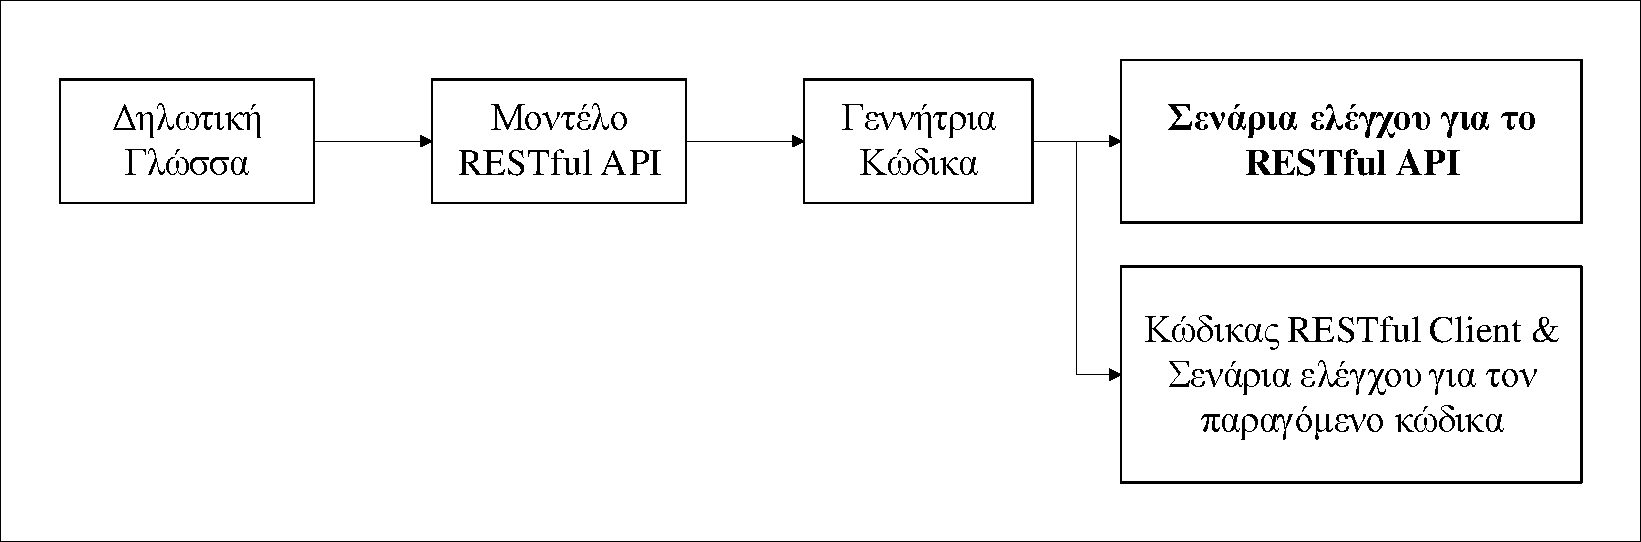
\includegraphics[width=\textwidth]{figures/DSL.pdf} 
    \caption{Διάγραμμα ροής χρήσης εργασίας}
    \label{figure3.1}
\end{figure} 

\section{Δηλωτική γλώσσα ορισμού μοντέλων διεπαφών}

Βασικός σκοπός της εργασίας είναι να μπορεί οποιοσδήποτε προγραμματιστής να περιγράφει με απλό τρόπο
τα χαρακτηριστικά μιας προγραμματιστικής διεπαφής τύπου \en{REST}
και να παίρνει ένα σύνολο από σενάρια ελέγχου που την καλύπτουν κατά το δυνατό περισσότερο.
Για τον λόγο αυτό ορίστηκε μία δηλωτική γλώσσα ορισμού μοντέλων διεπαφών.
Μέσω αυτής, μπορεί κανείς να προσδιορίσει με σαφήνεια όλες τις παραμέτρους που υποστηρίζονται,
δίχως να απαιτείται να έχει γνώση του εσωτερικού τρόπου λειτουργίας της εργασίας
και πώς αυτή μοντελοποιεί τα δεδομένα.

Για παράδειγμα,
ας υποθέσουμε πως έχουμε μία προγραμματιστική διεπαφή τύπου \en{REST}
με διεύθυνση βάσης '\emph{\en{/observatory/api}}' και ετικέτα '\emph{\en{my test api}}'.
Έστω ότι αυτή η διεπαφή διαθέτει ένα τελικό σημείο διαπίστευσης χρηστών,
το οποίο υποστηρίζει μέσω της μεθόδου \en{POST} δύο παραμέτρους σώματος για όνομα χρήστη και κωδικό πρόσβασης
και σε περίπτωση επιτυχίας επιστρέφει απάντηση με κωδικό κατάστασης 201.

Ο τρόπος με τον οποίο εκφράζονται τα παραπάνω στοιχεία μέσω της δηλωτικής γλώσσας είναι ο ακόλουθος:

\selectlanguage{english}
\begin{lstlisting}
api {
\end{lstlisting}
\begin{lstlisting}[deletekeywords={api}]
    baseUrl '/test/api'
    label   'my test api'
    endpoint(/login) {
        label 'Endpoint login'
        description 'Endpoint for user login with username and password'
        method(POST) {
            request(URL) {
                withBodyParameter(username, String)
                withBodyParameter(password, String)
            }
            response(JSON) {
                withStatus(201) {
                    body 'Created'
                }
            }
        }
    }
}
\end{lstlisting}
\selectlanguage{greek}

Η δηλωτική γλώσσα ορισμού μοντέλων διεπαφών σχεδιάστηκε με γνώμονα την ακριβέστερη απεικόνιση των χαρακτηριστικών ενός \en{RESTful API}.
Κοιτώντας μία προγραμματιστική διεπαφή εκφρασμένη στη συγκεκριμένη γλώσσα 
μπορεί κανείς εύκολα να κατανοήσει τις λειτουργίες και τις δυνατότητές της.
Παράλληλα κάθε έκφραση της γλώσσας είναι ξεκάθαρη 
και δεν αφήνει αμφιβολίες στον προγραμματιστή ως προς τη χρήση της.

Στο τέλος του κεφαλαίου παρατίθεται η πλήρης γραμματική της γλώσσας.

\section{Μοντελοποίηση προγραμματιστικής διεπαφής τύπου \en{REST}}
Θεωρούμε ότι κάθε προγραμματιστική διεπαφή (\en{API}) περιλαμβάνει τουλάχιστον ένα τελικό σημείο (\en{endpoint}), 
που το καθένα έχει τις δικές του μεθόδους (\en{methods}).
Κάθε μέθοδος έχει από μία αίτηση (\en{request}) και μία απάντηση (\en{response}).
Μία αίτηση αποτελείται από κεφαλίδες (\en{headers}) και παραμέτρους (\en{parameters}), 
οι οποίες μπορεί να είναι είτε σώματος (\en{body}) είτε αιτήματος (\en{query}).
Από την άλλη,
μία απάντηση αποτελείται από κεφαλίδες και μία κατάσταση (\en{status}).

\begin{figure}[!b]
    \centering
	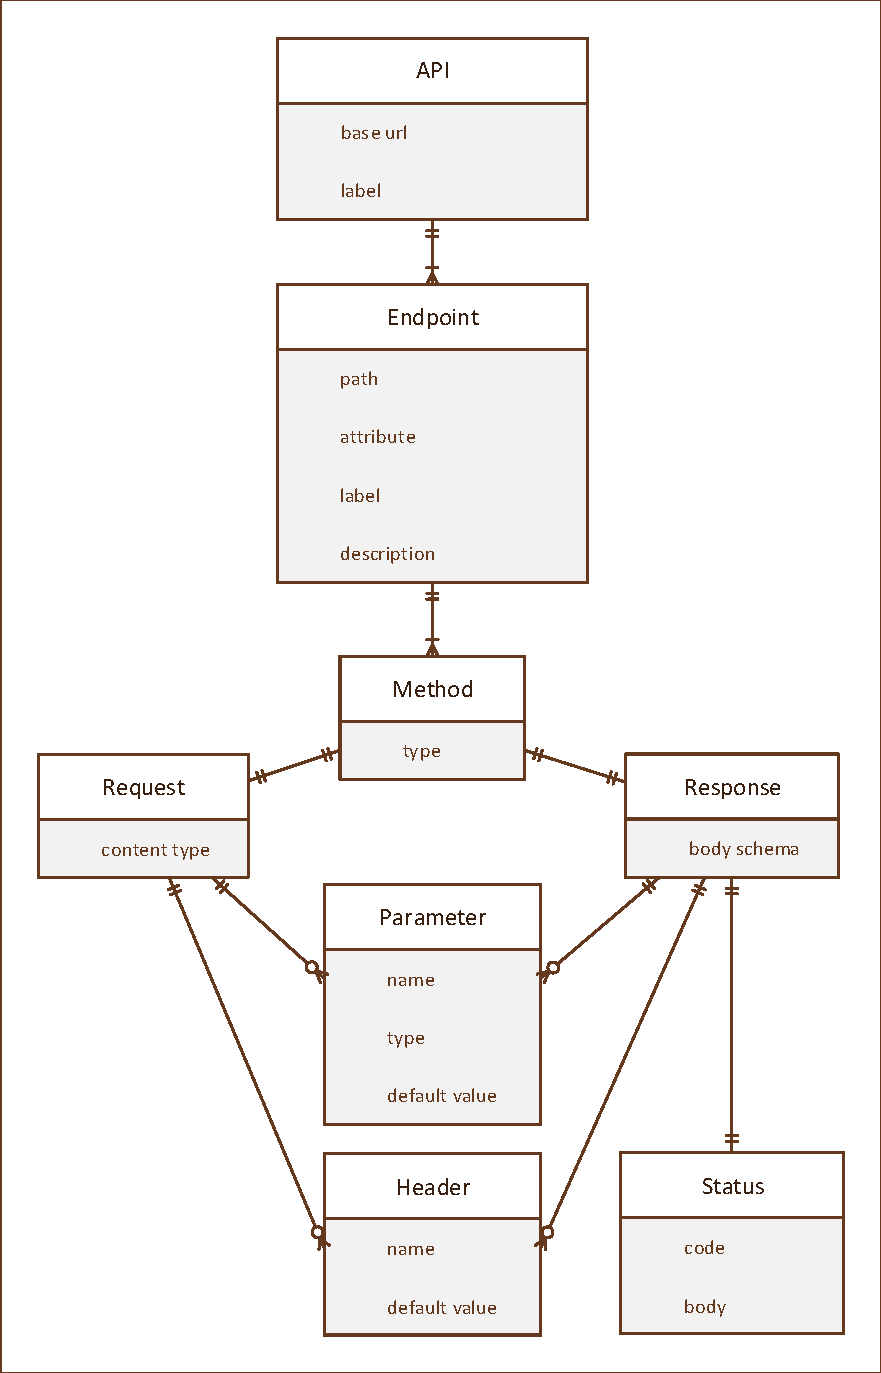
\includegraphics[height=18cm,keepaspectratio]{figures/ERD_eng.pdf} 
    \caption{Διάγραμμα οντοτήτων-συσχετίσεων}
    \label{figure3.2}
\end{figure} 

\begin{itemize}
    \item \underline{Προγραμματιστική Διεπαφή τύπου \en{REST} (\en{RESTful API})}
    
    Μία προγραμματιστική διεπαφή τύπου \en{REST},
    όπως περιγράφηκε και στο Κεφάλαιο 2,
    είναι ένα τμήμα λογισμικού ενός συστήματος
    που παρέχει σε προγραμματιστές πρόσβαση σε ένα σύνολο από λειτουργίες και διαδικασίες
    και ακολουθεί το αρχιτεκτονικό στυλ \en{REST (Representational State Transfer)}.

    Περιλαμβάνει:
    \begin{itemize}
        \item Μία διεύθυνση βάσης (\en{base URL}), όπως \en{https://api.example.com/}
        \item Μία ετικέτα (προαιρετικό), όπως '\en{API example}'
        \item Ένα τουλάχιστον τελικό σημείο (\en{endpoint})
    \end{itemize}

    
\item \underline{Τελικό Σημείο (\en{Endpoint})}

Ένα τελικό σημείο είναι ο δίαυλος επικοινωνίας μιας προγραμματιστικής διεπαφής με τον Παγκόσμιο Ιστό.

Είναι μία πύλη που επιτρέπει σε προγραμματιστές να στείλουν συγκεκριμένα αιτήματα προς τη διεπαφή και να τους επιστραφούν απαντήσεις.
Στην πράξη κάθε τελικό σημείο αναπαριστά μία ομάδα παρεμφερών λειτουργιών που υποστηρίζει η διεπαφή,
όπως αλληλεπίδραση με δεδομένα ή εκτέλεση εντολών.

Συνήθως ένα τελικό σημείο έχει το δικό του μονοπάτι που λειτουργεί ως πρόθεμα στη διεύθυνση της διεπαφής.

Περιλαμβάνει:
\begin{itemize}
    \item Ένα μονοπάτι
    \item Μία ετικέτα (προαιρετικό)
    \item Μία περιγραφή (προαιρετικό)
    \item Ένα ή περισσότερα προσδιοριστικά (προαιρετικά)
    \item Μία τουλάχιστον μέθοδο
\end{itemize}

\item \underline{Μέθοδος (\en{Method})}

Μία μέθοδος είναι μια επιθυμητή εντολή σε κάποιον πόρο του συστήματος.
Οι δυνατές εντολές είναι ορισμένες από το Πρωτόκολλο Μεταφοράς Υπερκειμένου (\en{HyperText Transfer Protocol, HTTP}) 
και δρουν σε ένα συγκεκριμένο τελικό σημείο της διεπαφής \cite{fielding1999hypertext}.
Σε αυτό μεταφέρουν ένα αίτημα και από αυτό δέχονται μία απάντηση.

Περιλαμβάνει:
\begin{itemize}
    \item Έναν τύπο
    \item Μία αίτηση
    \item Μία απάντηση
\end{itemize}

Στο πλαίσιο της εργασίας θεωρούμε ως επιτρεπτές τιμές του τύπου μιας μεθόδου τις \en{GET, POST, PUT, PATCH} και \en{DELETE}.

\item \underline{Αίτηση (\en{Request})}

Μία αίτηση είναι ένα μήνυμα που στέλνει ένας χρήστης ή ένα πρόγραμμα σε μια διεπαφή.
Αυτό το μήνυμα περιέχει όλες τις απαραίτητες πληροφορίες που χρειάζεται ο διακομιστής που θα την λάβει για να την διεκπεραιώσει.
Κάθε αίτηση πραγματοποιείται σε μια συγκεκριμένη διεύθυνση που συνήθως είναι ένα τελικό σημείο μιας διεπαφής.

Περιλαμβάνει:
\begin{itemize}
    \item Έναν τύπο περιεχομένου (\en{MIME})
    \item Ένα σύνολο από κεφαλίδες (προαιρετικό)
    \item Ένα σύνολο από παραμέτρους σώματος (προαιρετικό)
    \item Ένα σύνολο από παραμέτρους αιτήματος (προαιρετικό)
\end{itemize}

Ως τύπος περιεχομένου ορίζεται ένα αναγνωριστικό της μορφής 'τύπος/υπότυπος'
που περιγράφει τη μορφή του περιεχομένου της αίτησης.

Για τους σκοπούς της διπλωματικής,
οι τύποι περιεχομένου που υποστηρίζονται είναι αποκλειστικά οι '\en{application/json}' και '\en{application/x-www-form-urlencoded}'.

\item \underline{Απάντηση (\en{Response})}

Μία απάντηση είναι το αποτέλεσμα που παράγεται από μια διεπαφή που δέχεται μία αίτηση.
Δίνεται από το σύστημα που έχει την διεπαφή στον χρήστη ή το πρόγραμμα που στέλνει την αίτηση στο ίδιο τελικό σημείο που στάλθηκε αυτή.

Περιλαμβάνει:
\begin{itemize}
    \item Ένα σχήμα σώματος
    \item Ένα σύνολο από κεφαλίδες (προαιρετικό)
    \item Μία κατάσταση
\end{itemize}

Στο πλαίσιο της διπλωματική εργασίας
επιλέχθηκε η αναφορά του σχήματος του σώματος της απάντησης ως προαπαιτούμενο για την αυτόματη παραγωγή των αντιστοίχων σεναρίων ελέγχου.

Για την ακρίβεια, υποστηρίζονται οι μορφές \en{JSON}, συμβολοσειράς και ακεραίου αριθμού. 

\item \underline{Κεφαλίδα (\en{Header})}

Μία κεφαλίδα είναι το μέρος ενός μηνύματος αίτησης ή απάντησης 
που περιλαμβάνει πρόσθετες πληροφορίες επικοινωνίας.

Περιλαμβάνει:
\begin{itemize}
    \item Ένα όνομα
    \item Μία προεπιλεγμένη τιμή σε περίπτωση που είναι προαιρετική και δεν παρέχεται
\end{itemize}

Μία Κεφαλίδα πρέπει επίσης να δηλώνεται αν είναι υποχρεωτική ή προαιρετική.

\item \underline{Παράμετρος (\en{Parameter})}

Μία παράμετρος είναι ένα στοιχείο ενός μηνύματος
που βοηθάει στον προσδιορισμό παραμέτρων και στην μεταφορά πρόσθετων πληροφοριών.

Μπορεί να είναι είναι στο σώμα του μηνύματος, είτε στη διεύθυνση αιτήματος.

Περιλαμβάνει:
\begin{itemize}
    \item Ένα όνομα
    \item Έναν τύπο
    \item Μία προεπιλεγμένη τιμή σε περίπτωση που είναι προαιρετική και δεν παρέχεται
\end{itemize}

Μία παράμετρος πρέπει επίσης να δηλώνεται αν είναι υποχρεωτική ή προαιρετική.

\item \underline{Κατάσταση (\en{Status})}

Μία κατάσταση είναι το τμήμα της απάντησης που εκδίδεται από τον διακομιστή
και περιγράφει συνοπτικά το αποτέλεσμα της αίτησης.

Περιλαμβάνει:
\begin{itemize}
    \item Έναν κωδικό (πχ. 201)
    \item Ένα σώμα (πχ. '\en{Created}')
\end{itemize}

Ανάλογα με το είδος του αποτελέσματος της αίτησης,
έχουν καθιερωθεί οι ακόλουθες ομάδες κωδικών κατάστασης:

\begin{itemize}
    \item Ενημερωτικές απαντήσεις (100–199)
    \item Επιτυχείς απαντήσεις (200–299)
    \item Ανακατευθύνσεις (300–399)
    \item Προβλήματα χρήστη (400–499)
    \item Προβλήματα διακομιστή (500–599)
\end{itemize}

\end{itemize}

\section{Σενάρια ελέγχου της μοντελοποίησης}
Για να είμαστε βέβαιοι πως η υλοποίηση των παραπάνω αντικειμένων δεν έχει λάθη,
σχεδιάστηκαν σενάρια ελέγχου για καθένα από αυτά.
Έτσι, για κάθε αντικείμενο ελέγχουμε αν τα δεδομένα που του δίνουμε κατά τη δημιουργία 
είναι ίδια με αυτά που επιστρέφονται από αυτό που έχει παραχθεί.

Επιπλέον ελέγχουμε αν έχουν δοθεί τα υποχρεωτικά χαρακτηριστικά,
τα οποία ανάλογα την προδιαγραφή είναι:

\begin{itemize}
    \item Για την διεπαφή απαιτείται τουλάχιστον ένα τελικό σημείο.
    \item Για το τελικό σημείο απαιτείται το μονοπάτι και τουλάχιστον μία υποστηριζόμενη μέθοδος.
    \item Για τη μέθοδο απαιτούνται ο τύπος της, η αίτηση και η απάντηση.
    \item Για την απάντηση απαιτείται η κατάστασή της.
    \item Για την κεφαλίδα απαιτείται το όνομά της, ενώ σε περίπτωση που είναι υποχρεωτική απαιτείται και ένα προκαθορισμένο σώμα.
    \item Για την παράμετρο απαιτούνται το όνομά της και ο τύπος της, ενώ σε περίπτωση που είναι υποχρεωτική απαιτείται και ένα προκαθορισμένο σώμα.
    \item Τέλος, για την κατάσταση απαιτούνται ο κωδικός και το σώμα της.
\end{itemize}

Υπάρχουν ορισμένοι επιπρόσθετοι έλεγχοι για την ορθότητα των δεδομένων.
Έτσι, σε μία προγραμματιστική διεπαφή ελέγχουμε αν η διεύθυνση βάσης είναι έγκυρη διεύθυνση του Παγκοσμίου Ιστού
και σε μία κατάσταση αν ο κωδικός είναι εντός των υποστηριζόμενων ορίων (100-599).

\section{Γεννήτρια Κώδικα}
Έχοντας ορίσει αναλυτικά τις προδιαγραφές μιας διεπαφής προγραμματισμού τύπου \en{REST},
σχεδιάστηκε μία γεννήτρια κώδικα που λειτουργεί ως επεξεργαστής προτύπων.
Ένας επεξεργαστής προτύπων είναι ένα λογισμικό που συνδυάζει πρότυπα και μοντέλα δεδομένων 
με σκοπό την παραγωγή ενός τελικού κειμένου \cite{niemeyer2005learning}.

Η γεννήτρια κώδικα που σχεδιάστηκε χρησιμοποιεί ως μοντέλο δεδομένων την αναπαράσταση μιας διεπαφής
με τα χαρακτηριστικά που ορίστηκαν παραπάνω. 

Με τα πρότυπα που σχεδιάστηκαν,
η γεννήτρια κώδικα παράγει τα ακόλουθα:

\subsection{Πελάτης (\en{Client}) \en{RESTful API}}

Ο πελάτης διεπαφής είναι ένα λογισμικό που αξιοποιεί το πρωτόκολλο επικοινωνίας \en{HTTP}.
Με αυτό μπορούν να πραγματοποιηθούν όλες οι μορφές επικοινωνίας που δηλώνονται στις προδιαγραφές μιας διεπαφής.
Για τη διπλωματική εργασία είναι ένα απαραίτητο εργαλείο 
που στόχο έχει την εκτέλεση των τμημάτων των σεναρίων ελέγχου
που αφορούν την επικοινωνία με μία προγραμματιστική διεπαφή τύπου \en{REST}.

Για να το δημιουργήσει η γεννήτρια κώδικα,
αρχικά διαβάζει από τις προδιαγραφές της διεπαφής τη διεύθυνση βάσης,
καθώς και όλα τα τελικά σημεία που υποστηρίζονται.
Για καθένα από αυτά,
ελέγχει αν χρησιμοποιεί κάποιο προσδιοριστικό, 
καθώς και ποιες μεθόδους υποστηρίζει.
Λαμβάνεται υπόψη ακόμα και το σχήμα σώματος της απάντησης κάθε μεθόδου.  

\subsection{Σενάρια ελέγχου για τον παραγόμενο κώδικα με εικονικό διακομιστή (\en{Mock Server})}

Τα σενάρια ελέγχου με εικονικό διακομιστή είναι απαραίτητα για να βεβαιωθούμε πως ο πελάτης διεπαφής που θα δημιουργηθεί
θα εμφανίζει την επιθυμητή συμπεριφορά.

Η γεννήτρια κώδικα,
έχοντας παράξει τον πελάτη, 
χρησιμοποιεί τις προδιαγραφές της διεπαφής και
συντάσσει μια σειρά από σενάρια ελέγχου που περιλαμβάνουν την αποστολή και λήψη μηνυμάτων 
μέσα από τον πελάτη. 

Αρχικά αναλύει κάθε τελικό σημείο ως προς τις μεθόδους που υποστηρίζει,
ενώ παράλληλα ελέγχει αν χρησιμοποιεί κάποιο προσδιοριστικό.

Στη συνέχεια, προετοιμάζει μια εικονική αίτηση που θα χρησιμοποιηθεί για τους σκοπούς του ελέγχου.
Αυτή προκύπτει από τις προδιαγραφές της αίτησης κάθε μεθόδου και πιο συγκεκριμένα από τα παρακάτω στοιχεία:

Ανάλογα με τον τύπο περιεχομένου της αίτησης και πιο συγκεκριμένα αν αυτός είναι '\en{application/json}' ή '\en{application/x-www-form-urlencoded}',
παράγεται ένα αρχείο \en{JSON} ή μια συμβολοσειρά της μορφής '\en{field1=value1\&field2=value2}' με ζεύγη ονομάτων παραμέτρων και τιμών αντίστοιχα.
Σε κάθε περίπτωση περιλαμβάνονται τιμές για κάθε παράμετρο σώματος που υποστηρίζεται.

Με όμοιο τρόπο σχηματίζονται τιμές για κάθε κεφαλίδα και κάθε παράμετρο αίτησης σε μορφή πινάκων κατατεμαχισμού (\en{hashmap}).

Όπου χρειάζεται να μπει τιμή μεταβλητής σε παραμέτρους και κεφαλίδες,
έχουν επιλεγεί για τους σκοπούς της διπλωματικής εργασίας οι εξής τιμές:

\begin{itemize}
    \item Για συμβολοσειρές, τιμή της μορφής '\en{headerValue}'
    \item Για ακεραίους, ο αριθμός 42
    \item Για αριθμούς κινητής υποδιαστολής, ο αριθμός 42,5
    \item Για τύπους δεδομένων Αληθείας (\en{Boolean}), η τιμή Αληθής/\en{True}
\end{itemize}

Σε μεθόδους τύπου \en{GET, PUT, PATCH} και \en{DELETE} που χρησιμοποιούν προσδιοριστικό,
αυτό θεωρείται πως είναι ακέραιος αριθμός και για τους σκοπούς των ελέγχουν του ανατίθεται η τιμή 2.

Αμέσως μετά προδιαγράφεται ένας εικονικός διακομιστής (\en{Mock Server}).
Η λειτουργία του είναι όταν δέχεται στη διεύθυνση του τελικού σημείου
αίτηση με την αντίστοιχη μέθοδο και με τις κεφαλίδες και τις παραμέτρους σώματος και αίτησης των προδιαγραφών,
τότε να επιστρέφει μία συγκεκριμένη απάντηση στον πελάτη.
Αυτή θα έχει την κατάσταση,
τις κεφαλίδες της
και το σώμα της κατάστασης.
Το τελευταίο επιλέγεται ανάλογα με τον τύπο σχήματος και μπορεί να είναι είτε της μορφής \en{JSON},
είτε συμβολοσειρά είτε ακέραιος.

Η διαδικασία αυτή επαναλαμβάνεται για κάθε μέθοδο κάθε τελικού σημείου της διεπαφής.

\subsection{Σενάρια ελέγχου για το \en{RESTful API}}

Τέλος, τα σενάρια ελέγχου για το μοντέλο \en{RESTful API} παράγονται με παρόμοιο τρόπο με τα προαναφερθέντα,
με βασική διαφορά την έλλειψη εικονικού διακομιστή.
Αντί για αυτόν, η γεννήτρια κώδικα συντάσσει σενάρια ελέγχου που πραγματοποιούν αιτήσεις στη διεύθυνση και τη θύρα που έχουν οριστεί από τον χρήστη
και επαληθεύουν το αποτέλεσμα που δέχεται ο πελάτης διεπαφής.

Οι αιτήσεις προετοιμάζονται με τον ίδιο τρόπο ακριβώς με παραπάνω,
λαμβάνοντας υπόψη όλα τα χαρακτηριστικά της διεπαφής.

Οι έλεγχοι καλύπτουν:
\begin{itemize}
    \item Την ομαλή λειτουργία του διακομιστή και την επιτυχή σύνδεση σε αυτόν μέσω της θύρας που δίνεται.
    \item Τη δυνατότητα αποστολής μιας αίτησης με τις παραμέτρους και τις κεφαλίδες που υποστηρίζονται.
    \item Αν η απάντηση έχει τη μορφή που αναμένεται.
    \item Την ύπαρξη στις κεφαλίδες της απάντησης των πεδίων που αναμένονται.
    \item Την αποτυχία μιας αίτησης σε περίπτωση που λείπει μία υποχρεωτική παράμετρος ή κεφαλίδα.
\end{itemize}

\section{Γραμματική δηλωτικής γλώσσας ορισμού μοντέλων διεπαφών}

\selectlanguage{english}
\begin{lstlisting}
API                 : '{' 'baseUrl' BASEURL ('label' LABEL)? (('endpoint(' PATH+ ')' | ('endpoint(' PATH ',' ATTRIBUTE ')') ENDPOINT)+ '}'

ENDPOINT            : '{' ('label' LABEL)? ('description' DESCRIPTION)? 'method(' METHODTYPE ')' METHOD+ '}'

METHOD              : '{' 'request(' REQUESTTYPE ')' REQUEST 'response(' RESPONSESCHEMA ')' RESPONSE '}'

REQUEST             : '{' ('withBodyParameter(' PARAMETER ')')?+
                          ('withQueryParameter(' PARAMETER ')')?+
                          ('withHeader(' HEADER ')')?+ '}'

RESPONSE            : '{' 'withStatus' STATUS ('withHeader(' HEADER ')')?+ '}'
STATUS              : '(' INT ')' '{' 'body' WORD '}'
PARAMETER           : '(' ( ΝΑΜΕ ',' TYPE | NAME ',' TYPE ',' DEFAULTVALUE )')'
HEADER              : '(' ( ΝΑΜΕ | NAME ',' DEFAULTVALUE )')'
BASEURL             : WORD
LABEL               : WORD
PATH                : '/' WORD
ATTRIBUTE           : WORD
METHODTYPE          : 'GET' | 'POST' | 'PUT' | 'PATCH' | 'DELETE'
REQUESTTYPE         : 'JSON' | 'URL'
RESPONSESCHEMA      : 'JSON' | 'String' | 'Integer'
NAME                : WORD 
TYPE                : WORD
DEFAULTVALUE        : WORD
INT                 : [0-9]+  
\end{lstlisting}
\selectlanguage{greek} % Σχεδιασμός
\chapter{Υλοποίηση}
\InitialCharacter{Σ}το κεφάλαιο αυτό παρουσιάζεται η υλοποίηση της εργασίας. 
Περιγράφεται το περιβάλλον στο οποίο αναπτύχθηκε και
αναλύονται οι γλώσσες και τα εργαλεία προγραμματισμού που επιλέχθηκαν.

\section{Ολοκληρωμένο Περιβάλλον Ανάπτυξης (\en{IDE})}
Η εργασία υλοποιήθηκε στο ολοκληρωμένο περιβάλλον ανάπτυξης \en{IntelliJ IDEA Ultimate 2020}\footnote{\en{https://www.jetbrains.com/idea/}}.
Αυτό είναι ένα λογισμικό ανάπτυξης εφαρμογών που περιλαμβάνει μεταξύ άλλων έναν επεξεργαστή πηγαίου κώδικα,
έναν μεταγλωττιστή και εξειδικευμένα πρόσθετα υποβοήθησης προγραμματισμού. 

Επιλέχθηκε το συγκεκριμένο πρόγραμμα εξαιτίας της καθολικής υποστήριξης των γλωσσών προγραμματισμού που επιλέχθηκαν
και των εργαλείων που χρησιμοποιηθήκαν.

\section{Γλώσσα Προγραμματισμού}
Η γλώσσα προγραμματισμού που επιλέχθηκε για την αναπαράσταση των προδιαγραφών μιας προγραμματιστικής διεπαφής τύπου \en{REST} είναι η \en{Java}.

Η \en{Java} είναι μία γλώσσα αντικειμενοστρεφούς προγραμματισμού 
που σχεδιάστηκε από τον \en{James Gosling} και κυκλοφόρησε από την \en{Sun Microsystems} το 1995.
Οι λόγοι προτίμησης της συγκεκριμένης γλώσσας συμπίπτουν με τους πρωταρχικούς στόχους δημιουργίας της 
και πιο συγκεκριμένα επειδή είναι ανεξάρτητη από την πλατφόρμα του εξυπηρετητή, 
περιλαμβάνει εργαλεία και βιβλιοθήκες διαδικτύου
και έχει σχεδιαστεί για να εκτελεί κώδικα από εξωτερικές πηγές με ασφάλεια \cite{gosling1995java}.

Στο πλαίσιο του αντικειμενοστρεφούς προγραμματισμού,
η \en{Java} χρησιμοποιεί την έννοια της κλάσης
για να προσδιορίζει μια κατηγορία αντικειμένων
και παράλληλα να περιγράφει τα χαρακτηριστικά και τις λειτουργίες τους \cite{arnold2000java}.
Αυτή ακριβώς η έννοια αξιοποιήθηκε για την περιγραφή των προδιαγραφών μιας προγραμματιστικής διεπαφής τύπου \en{REST}
όπως αυτές σχεδιάστηκαν στο Κεφάλαιο 3.

\subsection{Διεπαφές (\en{Interfaces})}
Οι διεπαφές της \en{Java} είναι σύνολα ορισμένων αλλά μη υλοποιημένων λειτουργιών και διαδικασιών.
Αυτές ονομάζονται μέθοδοι και υλοποιούνται από κάποια κλάση\footnote{\en{https://docs.oracle.com/javase/tutorial/java/concepts/interface.html}}.

Αρχικά, δημιουργήθηκαν διεπαφές (\en{interfaces}) για καθένα από τα αντικείμενα που χρησιμοποιηθήκαν,
δηλαδή την προγραμματιστική διεπαφή τύπου \en{REST},
το τελικό σημείο,
τη μέθοδο,
την αίτηση,
την απάντηση,
την κεφαλίδα,
την παράμετρο
και την κατάσταση.
Κάθε διεπαφή περιλαμβάνει τις απαραίτητες διαχειριστικές μεθόδους ανάλογα με τα χαρακτηριστικά της οντότητας που περιγράφει.
Καθεμιά από αυτές ορίζει τη δυνατότητα ενός αντικειμένου να επιστρέφει ως απάντηση στην κλήση της
το αντίστοιχο χαρακτηριστικό των προδιαγραφών. 

Για παράδειγμα, μία διεπαφή προγραμματιστικής διεπαφής περιλαμβάνει μεθόδους για τη διεύθυνση βάσης,
την ετικέτα της
και το σύνολο από τα τελικά σημεία της.

Για λόγους ευκολίας,
από τη στιγμή που η εργασία υποστηρίζει τους τύπους περιεχομένου '\en{application/json}' και '\en{application/x-www-form-urlencoded}',
ο περιορισμός αυτός μεταφέρθηκε στον κώδικα στο σημείο των διεπαφών.
Έτσι, πέρα από την γενική διεπαφή της αίτησης,
υπάρχουν δύο επιπλέον,
η \en{RequestJSON} και η \en{RequestURL} που έχουν προκαθορισμένο τον αντίστοιχο τύπο.
Αυτές είναι που χρησιμοποιούνται στην υπόλοιπη εργασία.

\subsection{Υλοποιήσεις (\en{Implementations})}
Μια κλάση στη \en{Java} θεωρείται ότι υλοποιεί μία διεπαφή όταν
περιλαμβάνει τις μεθόδους που έχουν οριστεί από αυτήν
και περιγράφει τον τρόπο που εκτελούνται από το αντικείμενο.

Επομένως για κάθε διεπαφή δημιουργήθηκε μία αντίστοιχη κλάση,
η οποία υλοποιεί όλες τις μεθόδους και επιπλέον
περιέχει μεταβλητές για τα επιμέρους χαρακτηριστικά της,
καθώς και μία συνάρτηση δόμησης (\en{constructor}). 

Οι κλάσεις ακολουθούν την τεχνική της ενθυλάκωσης (\en{encapsulation}).
Πιο συγκεκριμένα, τα ευαίσθητα δεδομένα των μεταβλητών προστατεύονται από
τις μεθόδους της κλάσης, οι οποίες τα διαχειρίζονται και 
επιτρέπουν την πρόσβαση σε αυτά μόνο για ανάγνωση και όχι για επεξεργασία. 

Όλες οι μεταβλητές των κλάσεων που υλοποιούν διεπαφές είναι ιδιωτικές (\en{private}),
που σημαίνει πως πρόσβαση σε αυτές έχουν μόνο οι μέθοδοι της ίδιας κλάσης.

Αντίθετα, οι διαχειριστικές μέθοδοι που υλοποιούνται είναι όλες δημόσιες (\en{public}).
Αυτό σημαίνει πως ένα αντικείμενο μπορεί να μεταβιβάσει σε οποιοδήποτε άλλο αντικείμενο,
είτε ίδιας είτε διαφορετικής κλάσης,
πληροφορίες για τα χαρακτηριστικά του,
χωρίς όμως να δίνει πρόσβαση στις ίδιες τις μεταβλητές,
κάτι που θα εγκυμονούσε κινδύνους ασφαλείας και προβλήματα αστάθειας.

Για παράδειγμα,
η κλάση που υλοποιεί τη διεπαφή της προγραμματιστικής διεπαφής τύπου \en{REST}
περιλαμβάνει τις ιδιωτικές μεταβλητές της συμβολοσειράς διεύθυνσης βάσης, 
της συμβολοσειράς ετικέτας
και του συνόλου από αντικείμενα της κλάσης του τελικού σημείου.
Για τις τρεις αυτές ιδιωτικές μεταβλητές υπάρχουν οι αντίστοιχες δημόσιες μέθοδοι,
ίδιου τύπου,
χωρίς παραμέτρους,
που έχουν ως έξοδο στην κλήση τους τις αντίστοιχες μεταβλητές.
Τέλος, υπάρχει η δημόσια συνάρτηση δόμησης 
που δέχεται ως παραμέτρους τρεις μεταβλητές,
μία συμβολοσειρά για την διεύθυνση βάσης,
μία συμβολοσειρά για την ετικέτα
και ένα σετ από αντικείμενα τελικού σημείου για τα τελικά σημεία.
Η συνάρτηση αυτή χρησιμοποιείται για τη δημιουργία αντικειμένων της κλάσης της προγραμματιστικής διεπαφής τύπου \en{REST}
με χαρακτηριστικά που αντιστοιχούν στις μεταβλητές που δέχεται ως παραμέτρους.

\subsection{Σχεδιαστικό Πρότυπο}
Ως πρότυπο σχεδίασης της εργασίας επιλέχθηκε αυτό των κατασκευαστών (\en{builder pattern}).
Σκοπός του προτύπου σχεδίασης των κατασκευαστών είναι ο διαχωρισμός της διαδικασίας κατασκευής ενός σύνθετου αντικειμένου από την παρουσίασή του \cite{gamma1995design}.

Με άλλα λόγια,
για κάθε κλάση δημιουργήθηκε μία επιπλέον, 
ένας κατασκευαστής για αντικείμενα της αντίστοιχης κλάσης.
Ο κάθε κατασκευαστής, πέρα από ιδιωτικές μεταβλητές για τα χαρακτηριστικά του αντικειμένου που δημιουργεί,
περιέχει και δημόσιες μεθόδους που επιτρέπουν την επεξεργασία των μεταβλητών.
Αυτές δέχονται μέσω των ορισμάτων τους τιμές για τις αντίστοιχες μεταβλητές
και στο τέλος δημιουργούν ένα αντικείμενο με τα χαρακτηριστικά που έχει δώσει βήμα-βήμα ο προγραμματιστής 
ή το αντικείμενο που καλεί τον κατασκευαστή.

Στη συνάρτηση που δημιουργεί το τελικό αντικείμενο εμπεριέχονται και οι έλεγχοι
για την ορθότητά του με βάση τους περιορισμούς που ορίστηκαν κατά την σχεδίαση των αντικειμένων στο Κεφάλαιο 3.
Εφόσον τα δεδομένα που δέχεται ο κατασκευαστής δεν είναι έγκυρα,
η διαδικασία κατασκευής τερματίζεται και εγείρεται μήνυμα σφάλματος (\en{Runtime Exception}).
Αλλιώς καλείται η συνάρτηση δόμησης της αντίστοιχης κλάσης,
η οποία δέχεται ως ορίσματα τις μεταβλητές του κατασκευαστή με τις τελικές τιμές του,
όπως ορίστηκαν από τις μεθόδους του,
σε μορφή αμετάβλητων (\en{immutable}) αντικειμένων.

Για παράδειγμα, για τη δημιουργία ενός αντικειμένου της κλάσης της προγραμματιστικής διεπαφής τύπου \en{REST},
αρκεί να κληθεί ο αντίστοιχος κατασκευαστής με την εξής μορφή:

\selectlanguage{english}

\begin{lstlisting}[language=java]
    APISpecBuilder newApiBuilder = new APISpecBuilder();
    APISpec newAPI = newApiBuilder
                    .setLabel("api")
                    .setBaseUrl("https://www.example.com/api")
                    .addEndpoint(newEndpoint)
                    .build();
\end{lstlisting}

\selectlanguage{greek}

Με αυτόν τον τρόπο πετυχαίνουμε μεγαλύτερη ευχέρεια στην κατασκευή των αντικειμένων,
ενώ παράλληλα ισχυροποιείται ο έλεγχος που έχει ο προγραμματιστής κατά τη διαδικασία,
ελέγχοντας ταυτόχρονα την εγκυρότητα των δεδομένων.

Οι κατασκευαστές αντικειμένων που έχουν χαρακτηριστικά που αποτυπώνονται με σύνολα,
όπως για παράδειγμα μια προγραμματιστική διεπαφή που μπορεί να έχει πολλαπλά τελικά σημεία,
περιλαμβάνουν μεθόδους για την προσθήκη τόσο ενός από αυτά (πχ. \en{addEndpoint}) 
όσο και περισσοτέρων (πχ. \en{addEndpoints}).
Σε αντίθεση με τις μεθόδους για μεταβλητές που δέχονται μοναδική τιμή και αντικαθιστούν την τιμή με το όρισμα που δέχονται (πχ. \en{setBaseUrl}),
κάθε κλήση μιας μεθόδου προσθήκης δεδομένων διατηρεί τις υπάρχουσες τιμές του συνόλου και προσθέτει σε αυτές τα ορίσματά της.

\section{Κατασκευαστής \en{Groovy}}

Με βάση τη δηλωτική γλώσσα ορισμού μοντέλων διεπαφής που σχεδιάστηκε,
υλοποιήθηκε ένας κατασκευαστής που υποστηρίζει πλήρως τη γραμματική της.
Σκοπός του είναι να δέχεται από τον χρήστη την περιγραφή της διεπαφής για την οποία θέλει να παράξει σενάρια ελέγχου
και να δημιουργεί την αντίστοιχη μοντελοποίηση από αντικείμενα \en{Java}. 
Όπως βλέπουμε και στο σχήμα 4.1, 
στην είσοδό του δέχεται την δηλωτική περιγραφή ενός \en{RESTful API},
την οποία αναλύει με σκοπό να παράξει ένα \en{runtime} μοντέλο του,
δηλαδή στιγμιότυπα (\en{instances}) των κλάσεων \en{Java} που αναπαριστούν τα χαρακτηριστικά του.

Η γλώσσα προγραμματισμού που επιλέχθηκε για την υλοποίηση του συγκεκριμένου κατασκευαστή είναι η \en{Groovy}.
Η \en{Groovy} είναι και αυτή μία γλώσσα αντικειμενοστρεφούς προγραμματισμού,
παρόμοιου συντακτικού με την \en{Java}.
Ένα βασικό χαρακτηριστικό της γλώσσας \en{Groovy} που αξιοποιήθηκε για την εργασία 
είναι η υποστήριξη κομματιών κώδικα που λέγονται \en{closures}.
Ένα \en{closure} μπορεί να ανατεθεί σε μια μεταβλητή,
να δέχεται ορίσματα και να επιστρέφει τιμές.

Στον \en{Groovy} κατασκευαστή που υλοποιήθηκε (\en{Groovy Builder}),
χρησιμοποιήθηκαν ως \en{closures} οι περιγραφές που δίνει ο χρήστης για την προγραμματιστική διεπαφή του και τις ιδιότητές της.
Για παράδειγμα, 
ο ορισμός μιας διεπαφής γίνεται με την κλήση της συνάρτησης \en{api}(),
η οποία δέχεται ως όρισμα ένα \en{closure} στο οποίο περιλαμβάνονται 
η διεύθυνση βάσης, η ετικέτα και τα τελικά σημεία.

Ο τρόπος που θα κατασκευάζαμε μέσω του \en{Groovy Builder} μια προγραμματιστική διεπαφή 
με ένα τελικό σημείο διαπίστευσης χρηστών είναι ο ακόλουθος:

\selectlanguage{english}

\begin{lstlisting}
api {
\end{lstlisting}
\begin{lstlisting}[deletekeywords={api}]
    baseUrl '/test/api'
    label   'my test api'
    endpoint('/login') {
        label 'Endpoint login'
        description 'Endpoint for user login with username and password'
        method('POST') {
            request('URL') {
                withBodyParameter('username', 'String')
                withBodyParameter('password', 'String')
            }
            response('JSON') {
                withStatus(201) {
                    body 'Created'
                }
            }
        }
    }
}
\end{lstlisting}

\selectlanguage{greek}

Επιπλέον ο \en{Groovy Builder} δέχεται υποχρεωτικά ορισμένες πληροφορίες για αρχεία που παράγει η γεννήτρια κώδικα.
Οι πληροφορίες αυτές είναι οι τοποθεσίες, τα πακέτα και τα ονόματα 
του \en{REST API Client} και των σεναρίων ελέγχου,
καθώς και την θύρα (\en{port}) του \en{server} του χρήστη.

\subsection{Μέθοδοι}

\selectlanguage{english}

\begin{lstlisting}
baseUrl(String baseUrl) 
label(String label)
endpoint(String path, Closure configuration)
endpoint(String path, String attribute, Closure configuration)
description(String description)
method(String type, Closure configuration)
request(String type, Closure configuration) # type: JSON or URL
response(String schema, Closure configuration)
withBodyParameter(String name, String type)
withBodyParameter(String name, String type, Object defaultValueIfOptionalAndMissing)
withQueryParameter(String name, String type)
withQueryParameter(String name, String type, Object defaultValueIfOptionalAndMissing)
withHeader(String name)
withHeader(String name, String defaultValueIfOptionalAndMissing)
withStatus(Integer code, Closure configuration)
body(String body)
\end{lstlisting}

\selectlanguage{greek}

\subsection{Μεταβλητές}
\selectlanguage{english}
\begin{lstlisting}
// Rest API Client
clientFolder   # "/Project/src/main/java/"
clientPackage  # "app/restapiclient"
clientName     # "RestAPIClient"
serverPort     # 8765

// Rest API Server Tests
testFolder     # "/Project/src/test/groovy/"
testPackage    # "app/restapitests"
testName       # "TestServer"

// Rest API Client Tests with Mock Server
mockFolder     # "/Project/src/test/groovy/"
mockPackage    # "app/restapimocktests"
mockName       # "MockServer"
\end{lstlisting}
\selectlanguage{greek}


\begin{figure}
    \centering
	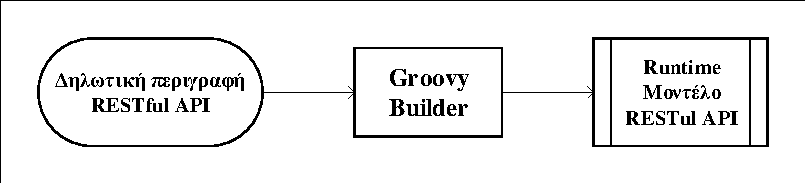
\includegraphics[width=\textwidth]{figures/groovy.pdf}
    \caption{Διάγραμμα ροής κατασκευαστή}
    \label{figure4.1}
\end{figure}

\section{Πλαίσιο Ελέγχου \en{Spock}}
Το \en{Spock} είναι ένα πλαίσιο ελέγχου για \en{Java} και \en{Groovy} εφαρμογές,
ικανό να διαχειριστεί τον πλήρη κύκλο ανάπτυξης ενός λογισμικού
συμβάλλοντας στην αυτοματοποίηση του ελέγχου \cite{kapelonis2016java}.

Με τη χρήση του εργαλείου \en{Spock} πραγματοποιούνται όλοι οι έλεγχοι στο πλαίσιο της εργασίας.
Ο τρόπος με τον οποίο γίνεται αυτό είναι ότι κάθε έλεγχος έχει τη μορφή ενός σεναρίου,
όπου δίνεται μία αρχική κατάσταση 
και παρατηρούμε αν ισχύουν οι συνθήκες που επιθυμούμε μετά την εκτέλεση ορισμένων εντολών. 

Πιο συγκεκριμένα,
για την αξιοποίησή του σε μία εφαρμογή \en{Java} πρέπει 
πρώτα να εισάγουμε την αντίστοιχη βιβλιοθήκη 
και μετά να δημιουργήσουμε κλάσεις \en{Groovy} που επεκτείνουν την '\emph{\en{spock.lang.Specification}}'.
Σε αυτές γράφουμε κομμάτια κώδικα ('\en{blocks}') που ακολουθούν τις φάσεις ('\en{phases}') \en{setup}, 
\en{stimulus}, \en{response} και \en{cleanup}.

Στη φάση \en{setup} ορίζονται οι αρχικές συνθήκες του σεναρίου, 
όπως οι μεταβλητές και τα αντικείμενα που θα χρησιμοποιηθούν στην πορεία.
Στις φάσεις \en{stimulus} και \en{response} περιλαμβάνεται ο κύριος κώδικας του ελέγχου,
όπου εκτελούνται μία ή περισσότερες ενέργειες και ελέγχονται τα αποτελέσματά τους.
Η τελευταία φάση \en{cleanup} αφορά απελευθέρωση πόρων του συστήματος 
και εκτελείται ακόμα κι αν προηγουμένως έχει εγερθεί κάποια εξαίρεση. 

Ο τρόπος με τον οποίο αποφασίζει το \en{Spock} αν ένα σενάριο ελέγχου επιτυγχάνει ή αποτυγχάνει
είναι να παρατηρεί τις συνθήκες που ορίζονται στη φάση \en{response} 
και που αφορούν τα δεδομένα που προκύπτουν από τη φάση \en{stimulus}.
Αν αυτές ικανοποιούνται όλες, 
τότε το σενάριο ελέγχου θεωρείται ότι επιτυγχάνει.
Αλλιώς, αν ακόμα και μία δεν ικανοποιείται, τότε αποτυγχάνει.

Ακολουθεί ένα παράδειγμα χρήσης του εργαλείου \en{Spock}.
Σε αυτό ελέγχουμε αν η διαδικασία αφαίρεσης ενός στοιχείου από μία λίστα ακεραίων αριθμών λειτουργεί σωστά.

\selectlanguage{english}
\begin{lstlisting}
def "Remove element from list"() {
    given:
        def list = [1, 2, 4, 8]

    when:
        list.remove(0)

    then:
        list == [2, 4, 8]
    }
\end{lstlisting}
\selectlanguage{greek}

Στο κομμάτι κώδικα '\en{given}' που αντιστοιχεί στη φάση \en{setup} ορίζουμε την αρχική κατάσταση του σεναρίου ελέγχου 
και πιο συγκεκριμένα δημιουργούμε μία λίστα με τέσσερις ακεραίους αριθμούς.
Στο κομμάτι κώδικα '\en{when}' που αντιστοιχεί στη φάση \en{stimulus} ορίζουμε την εντολή που θέλουμε να εκτελεστεί 
και της οποίας το αποτέλεσμα θέλουμε να ερευνήσουμε. Στην περίπτωσή μας είναι η αφαίρεση του πρώτου στοιχείου από τη λίστα.
Τέλος, στο κομμάτι κώδικα '\en{then}' που αντιστοιχεί στη φάση \en{response} ορίζουμε την συνθήκη που θέλουμε να ισχύει 
μετά το πέρας της εντολής αφαίρεσης, δηλαδή η λίστα να περιέχει πλέον όλα τα υπόλοιπα στοιχεία πέρα από το πρώτο που αφαιρέθηκε.

 
\section{Μηχανή Προτύπων \en{Freemarker}}
Η γεννήτρια κώδικα υλοποιήθηκε με χρήση της μηχανής προτύπων \en{Freemarker}.

Το \en{Freemarker} είναι μία μηχανή προτύπων (\en{Template Engine}) 
που χρησιμοποιείται ως βιβλιοθήκη της \en{Java}
με σκοπό την παραγωγή αρχείων κειμένου,
όπως στην περίπτωσή μας πηγαίος κώδικας.

Για τη λειτουργία της απαιτούνται έτοιμα κομμάτια κώδικα
που προσαρμόζουν τμήματά τους με βάση τα δεδομένα εισόδου της μηχανής προτύπων.
Αυτά τα κομμάτια κώδικα είναι γραμμένη σε μια συγκεκριμένη γλώσσα που ορίζει η βιβλιοθήκη
και τα δεδομένα που προσαρμόζονται λαμβάνονται από αντικείμενα \en{Java}.

Για παράδειγμα,
έστω ότι δίνουμε στη μηχανή προτύπων δώσουμε ένα αντικείμενο διεπαφής με διεύθυνση βάσης '\en{/my/api}'
και το πρότυπο περιλαμβάνει την ακόλουθη γραμμή:

\selectlanguage{english}
\begin{lstlisting}[deletekeywords={api,baseUrl}]
String BASE_URL = "${api.baseUrl}"
\end{lstlisting}
\selectlanguage{greek}

Τότε το παραγόμενο αρχείο θα αντικαταστήσει τη μεταβλητή με την τιμή που δίνει το αντικείμενο:

\selectlanguage{english}
\begin{lstlisting}[deletekeywords={api}]
String BASE_URL = "/my/api"
\end{lstlisting}
\selectlanguage{greek}

\section{Εργαλείο Κατασκευής Λογισμικού \en{Gradle}}
Το \en{Gradle} είναι ένα από τα πιο διαδεδομένα εργαλεία αυτοματοποίησης της κατασκευής λογισμικού.
Υποστηρίζει τις σχετικές διεργασίες όλων των σταδίων ανάπτυξης μιας εφαρμογής, 
από τη μεταγλώττιση του πηγαίου κώδικα μέχρι την εκτέλεση σεναρίων ελέγχου
και τη δημοσίευση του συστατικού (\en{artifact}) σε διαδικτυακές αποθήκες.
Υποστηρίζει πολλές γλώσσες προγραμματισμού,
με τις πιο δημοφιλείς να είναι η \en{Java}, η \en{C/C++} και η \en{JavaScript}.

Το \en{Gradle} λειτουργεί με σενάρια κατασκευής (\en{build scripts})
που περιλαμβάνουν όλα τα \en{projects} που αναλαμβάνει να αναπτύξει.
Κάθε \en{project} αποτελείται από εργασίες (\en{tasks}).
Αυτές είναι εντολές που μπορεί να αφορούν την εκτέλεση κώδικα,
τη μεταγλώττιση ενός προγράμματος και την είσοδο ή έξοδο αρχείων ή καταλόγων.

Για την οργάνωση των εργασιών που πρέπει να γίνουν,
το \en{Gradle} κατασκευάζει έναν κατευθυνόμενο άκυκλο γράφο (\en{DAG})
με βάση τις εξαρτήσεις τους.
Μέσα από τον γράφο καθορίζεται η προτεραιότητα των εργασιών,
καθώς κάθε εργασία για να πραγματοποιηθεί 
πρέπει πρώτα να έχουν ολοκληρωθεί όσες αντιστοιχούν σε προηγούμενους κόμβους.

Η διαδικασία κατασκευής του \en{Gradle} αποτελείται από τρεις φάσεις.
Στη φάση της αρχικοποίησης (\en{Initialization}) ρυθμίζεται το περιβάλλον εργασίας 
και εντοπίζονται τα \en{projects} που παίρνουν μέρος στη διαδικασία.
Στη φάση της διαμόρφωσης (\en{Configuration}) δημιουργείται ο γράφος εργασιων 
και καθορίζεται η σειρά εκτέλεσής τους.
Τέλος, στη φάση εκτέλεσης (\en{Execution}) εκτελούνται οι εργασίες με βάση την προτεραιότητα που αποφασίστηκε πριν.

Για την οργάνωση των \en{projects},
το \en{Gradle} χρησιμοποιεί αρχεία με όνομα '\en{build.gradle}'.
Σε αυτά περιλαμβάνονται όλες οι απαραίτητες πληροφορίες για τις εργασίες του \en{Gradle},
όπως τα \en{plugins} που χρησιμοποιούνται,
τα συστατικά (\en{artifacts}) στα οποία υπάρχουν εξαρτήσεις, καθώς και τα αποθετήρια στα οποία βρίσκονται.
Στο αρχείο αυτό συμπεριλαμβάνονται και οι ορισμοί των εργασιών. 

Στο πλαίσιο της εργασίας,
ο \en{Groovy Builder} υλοποιήθηκε έτσι ώστε να μπορεί να χρησιμοποιηθεί ως ένα \en{Gradle plugin}.
Πιο συγκεκριμένα, 
για τη χρήση του σε ένα \en{project} πρέπει πρώτα να υπάρχει ο αντίστοιχος κώδικας σε έναν φάκελο με όνομα '\en{buildSrc}'.
Στη συνέχεια, 
ο χρήστης με τις παρακάτω εντολές εισάγει τον \en{Groovy Builder} ως \en{plugin}:

\selectlanguage{english}
\begin{lstlisting}[morekeywords={apply,plugin}]
apply plugin: GroovyApiSpecBuilder
\end{lstlisting}
\selectlanguage{greek}

Έπειτα αρκεί να γράψει τον κώδικα στη δηλωτική γλώσσα \en{DSL} που διαβάζει ο \en{Groovy Builder},
καθώς και να παραθέσει τις απαραίτητες πληροφορίες για τον διακομιστή και τους φακέλους αποθήκευσης.
Η παραγωγή των σεναρίων ελέγχου,
καθώς και του κώδικα \en{RESTful API} και των σεναρίων ελέγχου για τον παραγόμενο κώδικα,
πραγματοποιείται με την εντολή '\en{generate}'. % Υλοποίηση
\chapter{Επαλήθευση Ορθής Λειτουργίας}
\InitialCharacter{Σ}το κεφάλαιο αυτό παρουσιάζονται οι εφαρμογές σε δύο διαδικτυακά \en{RESTful APIs} 
που επαληθεύουν την ορθή λειτουργία των εργαλείων που αναπτύχθηκαν στο πλαίσιο της παρούσας εργασίας.

\section{Παρατηρητήριο τιμών}
Η πρώτη προγραμματιστική διεπαφή τύπου \en{REST} που χρησιμοποιήθηκε για την επαλήθευση της εργασίας 
είναι τμήμα μιας εφαρμογής παρατηρητηρίου τιμών.
Ο κώδικας είναι διαθέσιμος στο διαδίκτυο σε \en{github repository}\footnote{\en{https://github.com/PavlosSta/SoftEng}}.

Τα χαρακτηριστικά της διεπαφής είναι τα ακόλουθα:

\begin{itemize}
    \item \textbf{Διεύθυνση}
    
    Ως διεύθυνση βάσης χρησιμοποιείται το '\en{https://localhost:8765/observatory/api}'.

    Οι πόροι του συστήματος δίνονται από τα τελικά σημεία στη μορφή \en{\{baseURL\}/\{path-to-resource\}}.

    Έτσι για παράδειγμα το τελικό σημείο για τα προϊόντα είναι το \en{\{baseURL\}/products},
    ενώ για το προϊόν με κωδικό 12 το \en{\{baseURL\}/products/12}.

    \item \textbf{Διαπίστευση} 
    
    Το τελικό σημείο διαπίστευσης χρηστών έχει το μονοπάτι '\en{\{baseURL\}/login}'.

    Η μοναδική μέθοδος που υποστηρίζει είναι η \en{POST}.

    Δέχεται ως παραμέτρους σώματος το \en{username} και το \en{password}, 
    ενώ σε περίπτωση επιτυχούς σύνδεσης επιστρέφει ένα \en{authentication token}.
    Αυτό θα πρέπει να περιλαμβάνεται ως κεφαλίδα με όνομα '\en{X-OBSERVATORY-AUTH}'
    σε όποια αίτηση απαιτείται πιστοποίηση.

    \item \textbf{Αποσύνδεση} 
    
    Τπ τελικό σημείο αποσύνδεσης χρηστών έχει το μονοπάτι '\en{\{baseURL\}/logout}'.

    Η μοναδική μέθοδος που υποστηρίζει είναι η \en{POST}.
    
    Θα πρέπει να έχει προηγηθεί διαπίστευση,
    η οποία θα έχει επιστρέφει ένα \en{authentication token}.
    Αυτό θα πρέπει να περιλαμβάνεται στην αίτηση ως κεφαλίδα ταυτοποίησης με όνομα '\en{X-OBSERVATORY-AUTH}'
    και αν είναι έγκυρο,
    η απάντηση θα είναι ένα \en{JSON} της μορφής '\en{\{ "message": "OK" \}}'.

    \item \textbf{Προϊόντα}
    
    Το τελικό σημείο των προϊόντων έχει το μονοπάτι '\en{\{baseURL\}/products}'.

    Σε αυτό υποστηρίζονται οι ακόλουθες μέθοδοι:

    \begin{enumerate}
        \item \underline{\textbf{\en{GET}}: Επιστρέφεται η λίστα των προϊόντων}
        
        Υποστηριζόμενες παράμετροι (ως μέρος του \en{URL query}):

        \selectlanguage{english}
        \begin{itemize}
            \item start: Integer, default 0
            \item count: Integer, default 20
            \item status: String, default ACTIVE
            \item sort: String, default id|DESC
        \end{itemize}
        \selectlanguage{greek}

        Για παράδειγμα:
        
        \en{GET} \emph{\en{\{baseURL\}/products?start=0\&count=100\&sort=id|ASC\&status=ALL}}

        Η απάντηση είναι ένα αρχείο \en{JSON} που περιλαμβάνει τις εξής παραμέτρους:

        \selectlanguage{english}
        \begin{itemize}
            \item start: Integer
            \item count: Integer
            \item total: Integer
            \item products: List<Product>
        \end{itemize}
        \selectlanguage{greek}

        Οι τρεις πρώτες παράμετροι αφορούν τη σελίδοποίηση των αποτελεσμάτων,
        ενώ η τελευταία περιλαμβάνει μία λίστα με τα προϊόντα της αντίστοιχης σελίδας.

        Κάθε προϊόν είναι ένα αρχείο \en{JSON} με τις εξής παραμέτρους:
        \selectlanguage{english}
        \begin{itemize}
            \item id: String
            \item name: String
            \item description: String
            \item category: String
            \item tags: List<String>
            \item withdrawn: Boolean
        \end{itemize}
        \selectlanguage{greek}


        \item \underline{\textbf{\en{POST}}: Δημιουργείται νέο προϊόν}
        
        Οι πληροφορίες που απαιτούνται για τη δημιουργία ενός προϊόντος 
        διατυπώνονται ως παράμετροι σώματος στην αίτηση.
        Αυτές είναι το \en{name}, το \en{description}, το \en{category} και τα \en{tags}.

        Προαιρετική παράμετρος είναι το \en{withdrawn}.
        
        Η απάντηση στην αίτηση δημιουργίας ενός προϊόντος 
        είναι η πλήρης κωδικοποίηση των δεδομένων του,
        δηλαδή ένα αρχείο \en{JSON} με τις αντίστοιχες πληροφορίες.
    \end{enumerate}

    Επιπλέον υποστηρίζει προσδιοριστικό (\en{attribute}) για το \en{id} των προϊόντων,
    με μονοπάτι της μορφής '\en{\{baseURL\}/products/\{id}\}'. 

    Με το \en{id} υποστηρίζονται οι ακόλουθες μέθοδοι:

    \begin{enumerate}
        \item \underline{\textbf{\en{GET}}: Επιστρέφονται οι πληροφορίες του προϊόντος}
        
        Για παράδειγμα, \en{GET} \emph{\en{\{baseURL\}/products/2}}.

        Το αποτέλεσμα της αίτησης είναι ένα αρχείο \en{JSON}
        με τα δεδομένα του προϊόντος με το αντίστοιχο \en{id}.

        Αυτά όπως και στην περίπτωση της μεθόδου \en{GET} χωρίς προσδιοριστικό \en{id}
        είναι τα ακόλουθα:

        \selectlanguage{english}
        \begin{itemize}
            \item id: String
            \item name: String
            \item description: String
            \item category: String
            \item tags: List<String>
            \item withdrawn: Boolean
        \end{itemize}
        \selectlanguage{greek}

        \item \underline{\textbf{\en{PUT}}: Ενημερώνονται οι πληροφορίες του προϊόντος}
        
        Η αίτηση πρέπει να περιλαμβάνει δεδομένα για όλα τα στοιχεία του προϊόντος, 
        τα οποία αντικαθιστούν τα προηγούμενα (\en{Full Update}).

        Τα δεδομένα αυτά περιλαμβάνονται στην αίτηση ως παράμετροι σώματος.

        Η απάντηση είναι η πλήρης κωδικοποίηση των δεδομένων του προϊόντος,
        δηλαδή ένα αρχείο \en{JSON} με τις αντίστοιχες πληροφορίες.

        \item \underline{\textbf{\en{PATCH}}: Ενημερώνονται μερικώς οι πληροφορίες του προϊόντος}
        
        Σε αντίθεση με τη μέθοδο \en{PUT},
        η \en{PATCH} επιτρέπει τη μερική επεξεργασία ενός προϊόντος (\en{Partial Update}).

        Τα δεδομένα για τα στοιχεία εκείνα που θέλουμε να ενημερώσουμε
        περιλαμβάνονται στην αίτηση ως παράμετροι σώματος.

        Η απάντηση είναι η πλήρης κωδικοποίηση των δεδομένων του προϊόντος,
        δηλαδή ένα αρχείο \en{JSON} με τις αντίστοιχες πληροφορίες.

        \item \underline{\textbf{\en{DELETE}}: Διαγράφεται το προϊόν}
        
        Το προϊόν με το αντίστοιχο \en{id} 
        αποκτά την τιμή \en{withdrawn=true} αν η αίτηση γίνεται από Εθελοντή,
        αλλιώς διαγράφεται από τη βάση δεδομένων αν γίνεται από Διαχειριστή.

        Το αποτέλεσμα είναι ένα αρχείο \en{JSON} της μορφής \en{\{ "message": "OK" \}}.
    \end{enumerate}
\end{itemize}
    
    Για λόγους συντομίας θα επικεντρωθούμε στα παραπάνω τελικά σημεία,
    αγνοώντας τα καταστήματα και τις τιμές,
    που έχουν όμοια λειτουργία με τα προϊόντα.

    Ας δούμε πώς μπορούμε να δηλώσουμε τις παραπάνω προδιαγραφές της διεπαφής 
    με σκοπό της παραγωγή σεναρίων ελέγχου.
    
    Καταρχάς, η διεύθυνσή του δίνεται ως η '\en{https://localhost:8765/observatory/api}',
    επομένως δηλώνουμε την θύρα του διακομιστή και τη διεύθυνση βάσης με τις εξής εντολές:

    \selectlanguage{english}
    \begin{lstlisting}[deletekeywords={api}]
    baseUrl '/observatory/api'
    serverPort = 8765
    \end{lstlisting}
    \selectlanguage{greek}

    Το πρώτο τελικό σημείο που έχουμε είναι αυτό της διαπίστευσης χρηστών.
    Παρατηρούμε πως υποστηρίζει μόνο τη μέθοδο \en{POST},
    για την οποία η αίτηση είναι τύπου \en{URL}
    με κωδικοποιημένες τις παραμέτρους σώματος \en{username} και \en{password}.
    Σε περίπτωση επιτυχούς σύνδεσης,
    έχουμε μία απάντηση με κατάσταση με κωδικό 201 και σώμα '\en{Created}'.

    Όλα τα παραπάνω γράφονται στον \en{Groovy Builder} με τον ακόλουθο τρόπο:

    \selectlanguage{english}
    \begin{lstlisting}
    endpoint('/login') {
    \end{lstlisting}
    \begin{lstlisting}[deletekeywords={endpoint}]
        label 'login endpoint'
        description 'the endpoint for user login'
        method('POST') {
            request('URL') {
                withBodyParameter('username', 'String')
                withBodyParameter('password', 'String')
            }
            response('JSON') {
                withStatus(201) {
                    body 'Created'
                }
            }
        }
    }
    \end{lstlisting}
    \selectlanguage{greek}

    Με όμοιο τρόπο περιγράφεται και το τελικό σημείο της αποσύνδεσης,
    το οποίο βέβαια αντί για \en{username} και \en{password} απαιτεί 
    μία κεφαλίδα με όνομα '\en{X-OBSERVATORY-AUTH}'.

    \selectlanguage{english}
    \begin{lstlisting}
    endpoint('/logout') {
    \end{lstlisting}
    \begin{lstlisting}[deletekeywords={endpoint}]
        label 'logout endpoint'
        description 'the endpoint for user logout'
        method('POST') {
            request('URL') {
                withHeader('X-OBSERVATORY-AUTH')
            }
            response('JSON') {
                withStatus(201) {
                    body 'Created'
                }
            }
        }
    }
    \end{lstlisting}
    \selectlanguage{greek}

    Σχετικά με το τελικό σημείο των προϊόντων,
    θα πρέπει να το δηλώσουμε μία φορά ως \en{endpoint} χωρίς προσδιοριστικό
    και άλλη μία ως \en{endpoint} με \en{id}.
    
    Για την περίπτωση χωρίς αναγνωριστικό,
    βλέπουμε ότι υποστηρίζονται οι μέθοδοι \en{GET} και \en{POST}.
    Αυτές δέχονται \en{URL} αιτήσεις 
    και οι απαντήσεις τους είναι σε μορφή \en{JSON}.

    Λαμβάνοντας υπόψη τις παραμέτρους και τις κεφαλίδες,
    προκύπτει ο ακόλουθος κώδικας για τον \en{Groovy Builder}:

    \selectlanguage{english}
    \begin{lstlisting}
    endpoint('/products') {
    \end{lstlisting}
    \begin{lstlisting}[deletekeywords={endpoint,description}]
        label 'products endpoint'
        method('GET') {
            request('URL') {
                withQueryParameter('start', 'Integer', 0)
                withQueryParameter('count', 'Integer', 20)
                withQueryParameter('status', 'String', 'ACTIVE')
                withQueryParameter('sort', 'String', 'id%7CDESC')
            }
            response('JSON') {
                withStatus(200) {
                    body 'OK'
                }
            }
        }
        method('POST') {
            request('URL') {
                withHeader('X-OBSERVATORY-AUTH')
                withBodyParameter('name', 'String')
                withBodyParameter('description', 'String')
                withBodyParameter('category', 'String')
                withBodyParameter('tags', 'String')
                withBodyParameter('withdrawn', 'boolean')
            }
            response('JSON') {
                withStatus(201) {
                    body 'OK'
                }
            }
        }
    }
    \end{lstlisting}
    \selectlanguage{greek}

    Στη συνέχεια έχουμε την περίπτωση ενός συγκεκριμένου προϊόντος με βάση το προσδιοριστικό \en{id} του.

    Δηλώνοντας τη μεταβλητή '\en{id}' μαζί με το μονοπάτι του τελικού σημείου
    και λαμβάνοντας υπόψη τις παραμέτρους και τις κεφαλίδες,
    προκύπτει ο ακόλουθος κώδικας για \en{Groovy Builder}:

    \selectlanguage{english}
    \begin{lstlisting}
    endpoint('/products', 'id') {
    \end{lstlisting}
    \begin{lstlisting}[deletekeywords={endpoint,description}]
        label 'products endpoint'
        method('GET') {
            request('URL') {}
            response('JSON') {
                withStatus(200) {
                    body 'OK'
                }
            }
        }
        method('PUT') {
            request('URL') {
                withHeader('X-OBSERVATORY-AUTH')
                withBodyParameter('name', 'String')
                withBodyParameter('description', 'String')
                withBodyParameter('category', 'String')
                withBodyParameter('tags', 'String')
                withBodyParameter('withdrawn', 'boolean')
            }
            response('JSON') {
                withStatus(201) {
                    body 'Created'
                }
            }
        }
        method('PATCH') {
            request('URL') {
                withHeader('X-OBSERVATORY-AUTH')
                withBodyParameter('name', 'String')
                withBodyParameter('description', 'String')
                withBodyParameter('category', 'String')
                withBodyParameter('tags', 'String')
                withBodyParameter('withdrawn', 'boolean')
            }
            response('JSON') {
                withStatus(201) {
                    body 'Created'
                }
            }
        }
        method('DELETE') {
            request('URL') {
                withHeader('X-OBSERVATORY-AUTH')
            }
            response('JSON') {
                withStatus(201) {
                    body 'Created'
                }
            }
        }
    }
    \end{lstlisting}
    \selectlanguage{greek}

    Εκτελώντας την εντολή \emph{\en{generate}} στο \en{Gradle},
    έχοντας πρώτα ορίσει και τις επιθυμητές τοποθεσίες,
    παράγονται τα εξής αρχεία:
    
    \begin{itemize}
        \item \underline{\en{REST API Client}}
        
        Το πρώτο και βασικό αρχείο που παράγεται είναι ο πελάτης (\en{client}) της διεπαφής.
        Αυτός πέρα από βοηθητικές διαδικασίες περιλαμβάνει για κάθε τελικό σημείο συναρτήσεις που υποστηρίζουν όλες τις μεθόδους του,
        μαζί με παραμέτρους και κεφαλίδες εφόσον αυτές παρέχονται.
        
        Για παράδειγμα, 
        η συνάρτηση που αντιστοιχεί στη μέθοδο \en{POST} του τελικού σημείου διαπίστευσης ('\en{login}') είναι η εξής:

        \selectlanguage{english}
        \begin{lstlisting}[language=java]
public Map<String, Object> post_to_login_with_headers_and_queryParams(String input, Map<String, String> headers, Map<String, List<String>> queryParams) {

    if(queryParams.isEmpty()) {
        return sendRequestAndParseResponseBodyAsUTF8Text(
                () -> newPostRequest(urlPrefix + "/login", "application/x-www-form-urlencoded", HttpRequest.BodyPublishers.ofString(input), headers),
                ClientHelper::parseJsonObject
        );
    }
    else {
        String queryParamString = queryParamsToString(queryParams);
        return sendRequestAndParseResponseBodyAsUTF8Text(
                () -> newPostRequest(urlPrefix + "/login" + queryParamString, "application/x-www-form-urlencoded", HttpRequest.BodyPublishers.ofString(input), headers),
                ClientHelper::parseJsonObject
        );
    }
}
\end{lstlisting}
\selectlanguage{greek}


Με παρόμοιο τρόπο δημιουργούνται οι υπόλοιπες μέθοδοι, 
ενώ καθεμιά, ανάλογα τον τύπο της, αξιοποιεί τις παρακάτω βοηθητικές διαδικασίες:

\selectlanguage{english}
\begin{lstlisting}[language=java]
private HttpRequest newPostRequest(String url, String contentType, HttpRequest.BodyPublisher bodyPublisher, Map<String, String> headers) {

    return newRequest("POST", url, contentType, bodyPublisher, headers);
}

private HttpRequest newGetRequest(String url, Map<String, String> headers) {

    return newRequest("GET", url, "application/x-www-form-urlencoded", HttpRequest.BodyPublishers.noBody(), headers);
}

private HttpRequest newPutRequest(String url, String contentType, HttpRequest.BodyPublisher bodyPublisher, Map<String, String> headers) {

    return newRequest("PUT", url, contentType, bodyPublisher, headers);
}

private HttpRequest newPatchRequest(String url, String contentType, HttpRequest.BodyPublisher bodyPublisher, Map<String, String> headers) {

    return newRequest("PATCH", url, contentType, bodyPublisher, headers);
}

private HttpRequest newDeleteRequest(String url, Map<String, String> headers) {

    return newRequest("DELETE", url, "application/x-www-form-urlencoded", HttpRequest.BodyPublishers.noBody(), headers);
}

\end{lstlisting}
\selectlanguage{greek}

Κάθε μέθοδος για να πραγματοποιήσει μια αίτηση χρησιμοποιεί την παρακάτω κοινή διαδικασία:

\selectlanguage{english}
\begin{lstlisting}[language=java]  
private HttpRequest newRequest(String method, String url, String contentType,
                                HttpRequest.BodyPublisher bodyPublisher, Map<String, String> headers) {

    HttpRequest.Builder builder = HttpRequest.newBuilder();

    builder.method(method, bodyPublisher)
            .header(CONTENT_TYPE_HEADER, contentType);

    for (Map.Entry<String,String> entry : headers.entrySet())
        builder.header(entry.getKey(), entry.getValue());

    return builder
            .uri(URI.create(url))
            .build();
}
\end{lstlisting}
\selectlanguage{greek}

Τέλος,
η πραγματοποίηση της \en{HTTP} αίτησης 
και η λήψη της απάντησης γίνονται από την ακόλουθη διαδικασία:

\selectlanguage{english}
\begin{lstlisting}[language=java]
private Map<String, Object> sendRequestAndParseResponseBodyAsUTF8Text(Supplier<HttpRequest> requestSupplier,
                                                                        Function<Reader, Map<String, Object>> bodyProcessor) {

    HttpRequest request = requestSupplier.get();

    Map<String, Object> bodyHeaders = new HashMap<>();

    try {
        System.out.println("Sending " + request.method() + " to " + request.uri());
        HttpResponse<InputStream> response = client.send(request, HttpResponse.BodyHandlers.ofInputStream());
        int statusCode = response.statusCode();
        if (statusCode == 200 || statusCode == 201) {
            try {
                if (bodyProcessor != null) {
                    bodyHeaders.put("headers", response.headers().map());
                    bodyHeaders.put("body", bodyProcessor.apply(new InputStreamReader(response.body(), StandardCharsets.UTF_8)));
                    return bodyHeaders;
                }
                else {
                    return null;
                }
            }
            catch(Exception e) {
                throw new ResponseProcessingException(e.getMessage(), e);
            }
        }
        else {
            throw new ServerResponseException(statusCode, ClientHelper.readContents(response.body()));
        }
    }
    catch(IOException | InterruptedException e) {
        throw new ConnectionException(e.getMessage(), e);
    }
}  
\end{lstlisting}
\selectlanguage{greek} 

Η παραπάνω διαδικασία υποστηρίζει αιτήσεις που έχουν μορφή \en{JSON}.
Με όμοιο τρόπο παράγονται για \en{String} και για \en{Integer}.
        
        \item \underline{Σενάρια ελέγχου για τον παραγόμενο κώδικα}
        
        Μαζί με τον παραπάνω \en{REST API Client},
        παράγονται και τα κατάλληλα σενάρια ελέγχου για αυτόν σε γλώσσα \en{Spock}.

        Για παράδειγμα, για το τελικό σημείο διαπίστευσης και τη μέθοδο \en{POST} που υποστηρίζει,
        δημιουργείται το παρακάτω σενάριο ελέγχου:
\selectlanguage{english}
\begin{lstlisting}[deletekeywords={api,body}]
def "POST to login with headers and queryParams"() {
    given:
    String requestBody = "username=bodyParamValue&password=bodyParamValue"
    ObjectMapper responseMapper = new ObjectMapper()
    JsonNode resultJSON = responseMapper.readTree("{\"value\":\"ok\"}")
    wms.givenThat(
            post(urlMatching("/observatory/api/login\\\\?.*"))
            .withRequestBody(containing(requestBody))
            .willReturn(aResponse()
                    .withStatus(201)
                    .withJsonBody(resultJSON)
            )
    )
    Map<String, String> headers = new HashMap<>()
    Map<String, List<String>> queryParams = new HashMap<>()

    when:
    Map<String, Object> result = caller.post_to_login_with_headers_and_queryParams(requestBody, headers, queryParams)

    then:
    result.get("body").toString().matches("[\\{\\[].*[\\}\\]]")
}
\end{lstlisting}
\selectlanguage{greek} 

Βλέπουμε ότι προσδιορίζεται ένας εικονικός διακομιστής (\en{Mock Server}),
που λαμβάνει τις αιτήσεις του \en{REST API Client}
με βάση μία κανονική έκφραση (\en{regular expression}) που ελέγχει τη διεύθυνση.

Παράλληλα δημιουργούνται δοκιμαστικές αιτήσεις με βάση τις ιδιότητες της μεθόδου και του τελικού σημείου.
Στο παράδειγμά μας οι παράμετροι σώματος '\en{username}' και '\en{password}' παίρνουν τυχαίες τιμές 
και αποκτούν την κωδικοποιημένη μορφή \en{URL}.

Ο εικονικός διακομιστής αναμένει αίτηση που περιλαμβάνει το περιεχόμενο που στέλνουμε
και επιστρέφει μία απάντηση με κωδικό κατάστασης 201 και ένα τυχαίο αρχείο \en{JSON}.

Ο τελευταίος έλεγχος αφορά την απάντηση που δέχεται ο \en{REST API Client} από τον εικονικό διακομιστή
και μέσω κανονικής έκφρασης ελέγχει αν είναι μορφής \en{JSON}. 


        \item \underline{Σενάρια ελέγχου για το \en{RESTful API}}
        
        Το τελευταίο αρχείο που παράγεται περιλαμβάνει σενάρια ελέγχου για τον '\en{RESTful API}',
        αυτή τη φορά θεωρώντας πως έχουμε πραγματικό διακομιστή αντί για εικονικό.
\selectlanguage{english}
\begin{lstlisting}[deletekeywords={body}]
def "POST to login with headers and queryParams"() {

    given:
    String requestBody = "username=bodyParamValue&password=bodyParamValue"
    Map<String, String> headers = new HashMap<>()
    Map<String, List<Object>> queryParams = new HashMap<>()

    when:
    Map<String, Object> result = caller.post_to_login_with_headers_and_queryParams(requestBody, headers, queryParams)
    Map<String, Object> resultHeaders = result.get("headers") as Map<String, Object>

    then:
    println("Body:")
    println(result.get("body"))
    println("Headers:")
    println(resultHeaders)
    result.toString().matches("[\\{\\[].*[\\}\\]]")
}
\end{lstlisting}
\selectlanguage{greek} 

Όπως βλέπουμε,
παρότι λείπει ο εικονικός διακομιστής,
δημιουργούμε μία αίτηση με βάση τις παραμέτρους και τις κεφαλίδες που υποστηρίζονται.

Στα σενάρια ελέγχου για το \en{RESTful API} έχουμε επιπλέον την εκτύπωση του σώματος και των κεφαλίδων της απάντησης.
Αυτό είναι χρήσιμες σε περιπτώσεις όπως αυτή του τελικού σημείου διαπίστευσης,
μιας και ο χρήστης μπορεί εύκολα να αντικαταστήσει τις προκαθορισμένες τιμές με ένα λειτουργικό ζεύγος 
\en{username} και \en{password} και να πάρει το \en{authentication token} είτε αυτό επιστρέφεται 
μέσω του σώματος της απάντησης,
είτε μέσω κάποιας κεφαλίδας της.

Εκτελώντας το παραπάνω σενάριο ελέγχου,
έχουμε την ακόλουθη έξοδο στην κονσόλα:

\selectlanguage{english}
\begin{lstlisting}[deletekeywords={api}]
Sending POST to https://localhost:8765/observatory/api/login
Body:
[token:$2a$10$hwOh6PJZeV1Nl9HKmOwsdO7RLWPxwEgojuYINKvDWwAYOkWvK11Uu]
Headers:
[content-length:[75], content-type:[application/json], date:[Mon, 11 Jan 2021 10:13:41 GMT], vary:[Origin, Access-Control-Request-Method, Access-Control-Request-Headers]]
\end{lstlisting}
\selectlanguage{greek} 

Επιπλέον παράγονται έλεγχοι για κάθε παράμετρο και κεφαλίδα που είναι υποχρεωτικές.
Στην περίπτωσή μας και οι δύο παράμετροι σώματος της αίτησης (\en{username} και \en{password}) είναι υποχρεωτικές.
Επομένως το ακόλουθο σενάριο ελέγχου πραγματοποιεί μία αίτηση χωρίς \en{username}
και θεωρείται έγκυρο αν ο διακομιστής εγείρει εξαίρεση.

\selectlanguage{english}
\begin{lstlisting}
def "POST to login without mandatory bodyParam: username"() {

    given:
    String requestBody = "password=bodyParamValue"
    Map<String, String> headers = new HashMap<>()
    Map<String, List<Object>> queryParams = new HashMap<>()

    when:
    caller.post_to_login_with_headers_and_queryParams(requestBody, headers, queryParams)

    then:
    thrown RuntimeException
}
\end{lstlisting}
\selectlanguage{greek} 
    \end{itemize}

\section{Ψηφιακό μητρώο δικτυακών υποδομών}
Η δεύτερη προγραμματιστική διεπαφή τύπου \en{REST} που χρησιμοποιήθηκε για την επαλήθευση της εργασίας
είναι τμήμα ενός ψηφιακού μητρώου για της δικτυακές υποδομές μιας χώρας.
Σκοπός του είναι η καταγραφή και η παρακολούθηση της κατάστασης
του συνόλου των διαθέσιμων δικτυακών υποδομών της χώρας.

Πιο συγκεκριμένα, η διεπαφή έχει τα εξής χαρακτηριστικά:

\begin{itemize}
    \item \textbf{Διεύθυνση}
    
    Ως διεύθυνση βάσης χρησιμοποιείται το '\en{https://localhost:44349/api}'.

    Οι πόροι του συστήματος δίνονται από τα τελικά σημεία στη μορφή \en{\{baseURL\}/\{path-to-resource\}}.

    Έτσι το τελικό σημείο των παρόχων είναι το \en{\{baseURL\}/NationalNetwork},
    ενώ για τον πάροχο με κωδικό 3 το \en{\{baseURL\}/NationalNetwork/3}.

    \item \textbf{Διαπίστευση} 
    
    Το τελικό σημείο διαπίστευσης χρηστών έχει το μονοπάτι '\en{\{baseURL\}/login}'.

    Η μοναδική μέθοδος που υποστηρίζει είναι η \en{POST}.

    Υπάρχουν δύο ειδών χρήστες στο σύστημα,
    οι Διαχειριστές που έχουν δικαίωμα επεξεργασίας όλων των δεδομένων
    και οι Πάροχοι που έχουν δικαίωμα επεξεργασίας μόνο των πληροφοριών των συνδέσεων.

    Το τελικό σημείο της διαπίστευσης δέχεται ένα αρχείο \en{JSON} με το \en{username} και το \en{password}.
    Σε περίπτωση επιτυχούς σύνδεσης επιστρέφει αρχείο \en{JSON} με το \en{id} του χρήστη,
    το \en{username} του, τον ρόλο του και ένα \en{Bearer token}.
    Αυτό θα πρέπει να περιλαμβάνεται ως κεφαλίδα ταυτοποίησης με όνομα '\en{Authorization}'
    σε όποια αίτηση απαιτείται πιστοποίηση.

    Η διάρκεια του \en{JSON Web Token} είναι 7 ημέρες.

    \item \textbf{Πάροχοι}
    
    Το τελικό σημείο των παρόχων έχει το μονοπάτι '\en{\{baseURL\}/NationalNetwork}'.

    Σε αυτό υποστηρίζονται οι ακόλουθες μέθοδοι:

    \begin{enumerate}
        \item \underline{\textbf{\en{GET}}: Επιστρέφεται η λίστα των παρόχων}
        
        Δικαίωμα προβολής των πληροφοριών των παρόχων έχει οποιοσδήποτε χρήστης,
        χωρίς ανάγκη πιστοποίησης.

        Η απάντηση είναι ένα αρχείο \en{JSON} που περιλαμβάνει μία λίστα με τα στοιχεία των παρόχων,
        της οποίας κάθε καταχώρηση περιλαμβάνει τις εξής παραμέτρους:

        \selectlanguage{english}
        \begin{itemize}
            \item id: Integer
            \item name: String
            \item location: String
            \item created: String
            \item email: String
        \end{itemize}
        \selectlanguage{greek}

        \item \underline{\textbf{\en{POST}}: Δημιουργείται νέα καταχώρηση παρόχου}
        
        Οι πληροφορίες που απαιτούνται για τη δημιουργία ενός παρόχου 
        διατυπώνονται ως παράμετροι σώματος στην αίτηση.
        Αυτές είναι το \en{name}, το \en{location} και το \en{email}.
        
        Η απάντηση στην αίτηση δημιουργίας ενός προϊόντος 
        είναι η πλήρης κωδικοποίηση των δεδομένων του,
        δηλαδή ένα αρχείο \en{JSON} με τις αντίστοιχες πληροφορίες.

    \end{enumerate}

    Επιπλέον υποστηρίζει προσδιοριστικό (\en{attribute}) για το \en{id} των παρόχων,
    με μονοπάτι της μορφής '\en{\{baseURL\}/NationalNetwork/\{id}\}'. 

    Με το \en{id} υποστηρίζονται οι ακόλουθες μέθοδοι:

    \begin{enumerate}
        \item \underline{\textbf{\en{GET}}: Επιστρέφονται οι πληροφορίες του παρόχου}
        
        Για παράδειγμα, \en{GET} \emph{\en{\{baseURL\}/products/2}}.

        Το αποτέλεσμα της αίτησης είναι ένα αρχείο \en{JSON}
        με τα δεδομένα του παρόχου με το αντίστοιχο \en{id}.

        Αυτά όπως και στην περίπτωση της μεθόδου \en{GET} χωρίς προσδιοριστικό \en{id}
        είναι τα ακόλουθα:

        \selectlanguage{english}
        \begin{itemize}
            \item id: Integer
            \item name: String
            \item location: String
            \item created: String
            \item email: String
        \end{itemize}
        \selectlanguage{greek}

        \item \underline{\textbf{\en{PATCH}}: Ενημερώνονται μερικώς οι πληροφορίες του παρόχου}
        
        Η μέθοδος \en{PATCH} επιτρέπει τη μερική επεξεργασία ενός παρόχου (\en{Partial Update}).

        Τα δεδομένα για τα στοιχεία εκείνα που θέλουμε να ενημερώσουμε
        περιλαμβάνονται στην αίτηση ως παράμετροι σώματος.

        Η απάντηση είναι η πλήρης κωδικοποίηση των δεδομένων του παρόχου,
        δηλαδή ένα αρχείο \en{JSON} με τις αντίστοιχες πληροφορίες.

        \item \underline{\textbf{\en{DELETE}}: Διαγράφεται ο πάροχος}
        
        Ο πάροχος με το αντίστοιχο \en{id} διαγράφεται από τη βάση δεδομένων,
        εφόσον η αίτηση γίνεται από χρήστη με ρόλο Διαχειριστή.

        Το αποτέλεσμα είναι ένα αρχείο \en{String} της μορφής \en{"success at deletion"}.
    \end{enumerate}
\end{itemize}

Για λόγους συντομίας θα ασχοληθούμε μόνο με το τελικό σημείο των παρόχων.
Όμοια με αυτό λειτουργούν τα τελικά σημεία των συνδέσεων και των χρηστών,
ενώ η διαπίστευση δε διαφέρει σημαντικά από αυτήν του παρατηρητηρίου τιμών του πρώτου παραδείγματος.

Η διεύθυνση της διεπαφής δίνεται ως η '\en{https://localhost:44349/api}',
επομένως δηλώνουμε την θύρα του διακομιστή και τη διεύθυνση βάσης με τις εξής εντολές:

\selectlanguage{english}
\begin{lstlisting}[deletekeywords={api}]
baseUrl '/api'
serverPort = 44349
\end{lstlisting}
\selectlanguage{greek}

Όπως και πριν,
έτσι και τώρα θα δηλώσουμε μία φορά το τελικό σημείο χωρίς προσδιοριστικό 
και μία με το \en{id}.

Μία βασική διαφορά των δύο διεπαφών είναι ότι το ψηφιακό μητρώο δικτυακών υποδομών
δέχεται αιτήσεις με τύπο περιεχομένου \en{JSON} αντί για \en{URL}.
Αυτό όμως δεν είναι πρόβλημα ούτε απαιτεί κάποια σημαντική αλλαγή πέρα από τη δήλωση '\en{JSON}' 
στην αίτηση κάθε μεθόδου.

Έτσι, για παράδειγμα, 
για να περιγράψουμε στον \en{Groovy Builder} το τελικό σημείο των παρόχων με και χωρίς προσδιοριστικό,
γράφουμε τα εξής:

\selectlanguage{english}
\begin{lstlisting}
endpoint('/NationalNetwork') {
\end{lstlisting}
\begin{lstlisting}[deletekeywords={endpoint}]
    label 'providers networks'
    description 'an endpoint for providers'
    method('GET') {
        request('JSON') {}
        response('JSON') {
            withStatus(200) {
                body 'OK'
            }
        }
    }
    method('POST') {
        request('JSON') {
            withHeader('Authorization')
            withBodyParameter('name', 'String')
            withBodyParameter('location', 'String')
            withBodyParameter('email', 'String')
        }
        response('JSON') {
                withStatus(201) {
                    body 'Created'
                }
        }
    }
}
\end{lstlisting}
\begin{lstlisting}
endpoint('/NationalNetwork', 'id') {
\end{lstlisting}
\begin{lstlisting}[deletekeywords={endpoint}]
    label 'providers networks with id'
    description 'an endpoint for providers by id'
    method('PATCH') {
        request('JSON') {
            withHeader('Authorization')
            withBodyParameter('name', 'String')
            withBodyParameter('location', 'String')
            withBodyParameter('email', 'String')
        }
        response('JSON') {
            withStatus(200) {
                body 'OK'
            }
        }
    }
    method('DELETE') {
        request('JSON') {
            withHeader('Authorization')
            withBodyParameter('name', 'String')
            withBodyParameter('location', 'String')
            withBodyParameter('email', 'String')
        }
        response('String') {
            withStatus(201) {
                body 'Created'
            }
        }
    }
}
\end{lstlisting}
\selectlanguage{greek}

Με την εκτέλεση της εντολής \emph{\en{generate}} στον \en{Gradle},
πάραγονται όπως και πριν τα παρακάτω τρία αρχεία:

\begin{itemize}
    \item \underline{\en{REST API Client}}
    
    Βλέπουμε ότι στον πελάτη που δημιουργείται, 
    για κάθε μέθοδο της διεπαφής που δέχεται αιτήσεις τύπου \en{JSON},
    αυτόματα αλλάζει το όρισμα του τύπου δεδομένων σε '\en{application/json}'.    

    \selectlanguage{english}
    \begin{lstlisting}[language=java]
    public Map<String, Object> post_to_NationalNetwork_with_headers_and_queryParams(String input, Map<String, String> headers, Map<String, List<String>> queryParams) {

        if(queryParams.isEmpty()) {
            return sendRequestAndParseResponseBodyAsUTF8Text(
                    () -> newPostRequest(urlPrefix + "/NationalNetwork", "application/json", HttpRequest.BodyPublishers.ofString(input), headers),
                    ClientHelper::parseJsonObject
            );
        }
        else {
        String queryParamString = queryParamsToString(queryParams);

            return sendRequestAndParseResponseBodyAsUTF8Text(
                    () -> newPostRequest(urlPrefix + "/NationalNetwork" + queryParamString, "application/json", HttpRequest.BodyPublishers.ofString(input), headers),
                    ClientHelper::parseJsonObject
            );
        }
    }
    \end{lstlisting}
    \selectlanguage{greek}

    \item \underline{Σενάρια ελέγχου για τον παραγόμενο κώδικα}

    Στα σενάρια ελέγχου που παράγονται και αφορούν τον κώδικα του \en{REST API Client}
    αυτή τη φορά έχουμε τελικό σημείο διαπίστευσης που δέχεται τα δεδομένα σε μορφή \en{JSON}.
    Δηλώνοντάς το αυτό στον \en{Groovy Builder},
    το αντίστοιχο σενάριο ελέγχου είναι το εξής:

    \selectlanguage{english}
    \begin{lstlisting}[deletekeywords={api,body}]
    def "POST to users_authenticate with headers and queryParams"() {

        given:
        String requestBody = new JSONObject()
            .put("username", "bodyParamValue")
            .put("password", "bodyParamValue")
            .toString();
        ObjectMapper responseMapper = new ObjectMapper()
        JsonNode resultJSON = responseMapper.readTree("{\"value\":\"ok\"}")
        wms.givenThat(
                post(urlMatching("/api/users/authenticate\\\\?.*"))
                .withRequestBody(containing(requestBody))
                .willReturn(aResponse()
                        .withStatus(201)
                        .withJsonBody(resultJSON)
                )
        )
        Map<String, String> headers = new HashMap<>()
        Map<String, List<String>> queryParams = new HashMap<>()
        
        when:
        Map<String, Object> result = caller.post_to_users_authenticate_with_headers_and_queryParams(requestBody, headers, queryParams)
        
        then:
        result.get("body").toString().matches("[\\{\\[].*[\\}\\]]")
    }
\end{lstlisting}
\selectlanguage{greek}

    \item \underline{Σενάρια ελέγχου για το \en{RESTful API}}
    
    Όμοια με παραπάνω,
    το σενάριο ελέγχου για την διαπίστευση των χρηστών προσαρμόζεται στα δεδομένα εισόδου 
    και γίνεται το ακόλουθο:

    \selectlanguage{english}
    \begin{lstlisting}[deletekeywords={body}]
    def "POST to users_authenticate with headers and queryParams"() {

        given:
        String requestBody = new JSONObject()
            .put("username", "bodyParamValue")
            .put("password", "bodyParamValue")
            .toString();
        Map<String, String> headers = new HashMap<>()
        Map<String, List<Object>> queryParams = new HashMap<>()

        when:
        Map<String, Object> result = caller.post_to_users_authenticate_with_headers_and_queryParams(requestBody, headers, queryParams)
        Map<String, Object> resultHeaders = result.get("headers") as Map<String, Object>

        then:
        println("Body:")
        println(result.get("body"))
        println("Headers:")
        println(resultHeaders)

        result.toString().matches("[\\{\\[].*[\\}\\]]")
    }
\end{lstlisting}
\selectlanguage{greek}

    Αυτή τη φορά μπορούμε να τροποποιήσουμε το σενάριο ελέγχου 
    αλλάζοντας τις τυχαίες τιμές των παραμέτρων \en{username} και \en{password} στο \en{JSON} αρχείο αίτησης
    με ένα ζεύγος έγκυρων δεδομένων.
    
    Το \en{authentication token} που θα τυπωθεί στην κονσόλα μπορούμε να το αντιγράψουμε 
    στην τιμή της αντίστοιχης κεφαλίδας πιστοποίησης των σεναρίων ελέγχου που την απαιτούν.
    
    Έτσι, για παράδειγμα, μπορούμε να αντικαταστήσουμε με αυτό το '\en{headerValue}' στο σενάριο ελέγχου της δημιουργίας 
    νέου παρόχου μέσω μεθόθου \en{POST}, το οποίο παράγεται αυτόματα ως εξής:

    \selectlanguage{english}
    \begin{lstlisting}[deletekeywords={body}]
def "POST to NationalNetwork with headers and queryParams"() {

    given:
    String requestBody = new JSONObject()
        .put("name", "bodyParamValue")
        .put("location", "bodyParamValue")
        .put("email", "bodyParamValue")
        .toString();
    Map<String, String> headers = new HashMap<>()
    headers.put("Authorization", 'headerValue')
    Map<String, List<Object>> queryParams = new HashMap<>()

    when:
    Map<String, Object> result = caller.post_to_NationalNetwork_with_headers_and_queryParams(requestBody, headers, queryParams)
    Map<String, Object> resultHeaders = result.get("headers") as Map<String, Object>

    then:
    println("Body:")
    println(result.get("body"))
    println("Headers:")
    println(resultHeaders)

    result.toString().matches("[\\{\\[].*[\\}\\]]")
}
\end{lstlisting}
\selectlanguage{greek}
    
\end{itemize} % Παραδείγματα Χρήσης
\chapter{Σχετικές Εργασίες}
\InitialCharacter{Η} μελέτη των προγραμματιστικών διεπαφών τύπου \en{REST} και του ελέγχου τους,
παρότι είναι ένας τομέας που αξιοποιείται σημαντικά σε επιχειρησιακό επίπεδο,
παρουσιάζει και μεγάλο ερευνητικό ενδιαφέρον σήμερα.

Οι προγραμματιστικές διεπαφές τύπου \en{REST} μελετώνται παράλληλα με τις σύγχρονες τεχνολογικές τάσεις,
όπως είναι για παράδειγμα η ανάπτυξη της νέας γενιάς ασύρματων δικτύων \en{5G} \cite{mayer2018restful}.
Η νέα γενιά αυτή αναμένεται να επιφέρει ραγδαίες εξελίξεις ως προς τη μετάβαση στο διαδίκτυο των πραγμάτων (\en{IoT}) \cite{wang2018iot},
μία κατάσταση στην οποία μηχανές και συσκευές καθημερινής χρήσης αλληλεπιδρούν μεταξύ τους 
μέσω ενος διεθνούς δικτύου \cite{gubbi2013internet}. 

Με την έκρηξη της μηχανικής μάθησης και των νευρωνικών δικτύων,
έχουν υπάρξει προσπάθειες αξιοποίησης της τεχνητής νοημοσύνης στον κλάδο των προγραμματιστικών διεπαφών.
Αυτές περιλαμβάνουν 
τόσο τη σχεδίαση νέων μορφών διεπαφών, προσαρμοσμένων στις απαιτήσεις της μηχανικής μάθησης \cite{garcia2019deepaas}\cite{howard2020fastai}
και την σύγκριση των δημοφιλέστερων \cite{kubany2020comparison},
όσο και τον έλεγχο των διεπαφών με την αυτοματοποιημένη παραγωγή μεγάλου όγκου σεναρίων ελέγχου 
που προκύπτουν από την ανάλυση χιλιάδων άλλων προγραμμάτων \cite{martin2020ai}.

Στο παρόν κεφάλαιο περιγράφονται τα παρακάτω πιο δημοφιλή εργαλεία που χρησιμοποιούνται σήμερα 
για την μοντελοποίηση και τον έλεγχο προγραμματιστικών διεπαφών τύπου \en{REST}:

\begin{itemize}
    \item \en{OpenAPI Specification} \cite{noauthor_oaiopenapispecification_2021}
    \item \en{Swagger Inspector} \cite{swagger}
    \item \en{Postman} \cite{postman}
\end{itemize}

\section{\en{OpenAPI Specification}}

Το \en{OpenAPI Specification} είναι μία προδιαγραφή μοντελοποίησης για \en{RESTful} διεπαφές προγραμματισμού 
που χρησιμοποιείται για την περιγραφή, την ανάπτυξη, τη χρήση και την αναπαράστασή τους.

Η προδιαγραφή \en{OpenAPI} είναι ανεξάρτητη από τη γλώσσα προγραμματισμού και επιτρέπει 
τόσο στους προγραμματιστές να περιγράψουν εύκολα και κατανοητά μια διεπαφή, 
όσο και σε εφαρμογές να αλληλεπιδράσουν μαζί της.

Η μορφή που έχει είναι ένα αρχείο \en{JSON}
που περιλαμβάνει τα υποστηριζόμενα πεδία με τις τιμές τους.
Οι τιμές αυτές μπορεί να δηλώνουν είτε μία σταθερά είτε ένα σχήμα δεδομένων.

Οι τύποι δεδομένων που υποστηρίζονται είναι οι εξής:

\begin{itemize}
    \item Αριθμοί (\en{integer}, \en{long}, \en{float}, \en{double})
    \item Συμβολοσειρές (συμπεριλαμβανομένων \en{bytes} και \en{bits})
    \item Tύποι δεδομένων Αληθείας (\en{Boolean})
    \item Ειδικοί τύποι δεδομένων, όπως ημερομηνίες και κωδικοί πρόσβασης
\end{itemize}

Το αρχείο \en{JSON} της προδιαγραφής μπορεί να περιλαμβάνει τα ακόλουθα πεδία:

\begin{itemize}
    \item \underline{\en{openapi}}
    
    Υποχρεωτικό πεδίο, περιλαμβάνει την έκδοση της προδιαγραφής \en{OpenAPI} που χρησιμοποιείται.

    \item \underline{\en{info}}
    
    Υποχρεωτικό πεδίο, περιλαμβάνει απαραίτητες πληροφορίες για την διεπαφή.

    \item \underline{\en{servers}}
    
    Περιλαμβάνει τους διακομιστές με τους οποίους επικοινωνεί η διεπαφή.

    \item \underline{\en{paths}}
    
    Υποχρεωτικό πεδίο, περιλαμβάνει τα μονοπάτια των τελικών σημείων και των λειτουργιών τους.
    
    \item \underline{\en{components}}
    
    Περιλαμβάνει όλα τα δομικά στοιχεία της διεπαφής.
    
    \item \underline{\en{security}}
    
    Περιλαμβάνει περιγραφές των μηχανισμών ασφαλείας της διεπαφής.

    \item \underline{\en{tags}}
    
    Περιλαμβάνει ετικέτες με μεταδεδομένα (\en{metadata}) για την διεπαφή.
    
    \item \underline{\en{externalDocs}}
    
    Περιλαμβάνει εξωτερικά έγγραφα τεκμηρίωσης.
\end{itemize}

Το κομμάτι που παρουσιάζει ενδιαφέρον για την παρούσα εργασία είναι εκείνο των δομικών στοιχείων (\en{components}).
Όπως φαίνεται, χρησιμοποιώντας την προδιαγραφή \en{OpenAPI},
μπορεί κανείς να ορίσει μία προγραμματιστική διεπαφή τύπου \en{REST} ως ένα σύνολο από τα ακόλουθα συστατικά:

\begin{itemize}
    \item \underline{\en{schemas}}
    
    Περιγραφές για τα δεδομένα εισόδου ή εξόδου. Αυτές μπορεί να είναι μία κανονική έκφραση (\en{regex}) του περιεχομένου,
    μέγιστο και ελάχιστο μήκος ή πλήθος αντικειμένων κλπ.

    \item \underline{\en{responses}}
    
    Λίστα με τις αναμενόμενες απαντήσεις με βάση την κωδικό κατάστασης (\en{HTTP status code}).
    
    Κάθε απάντηση περιλαμβάνει υποχρεωτικά περιγραφική (\en{description}), 
    ενώ προαιρετικά πληροφορίες για τις κεφαλίδες και το περιεχόμενό της, 
    όπως το σχήμα των δεδομένων.

    \item \underline{\en{parameters}}
    
    Η προδιαγραφή \en{OpenAPI} ορίζει τέσσερις τύπους παραμέτρων:

    \begin{enumerate}
        \item \en{path} - μονοπατιού διεύθυνσης
        \item \en{query} - επιθέματος διεύθυνσης
        \item \en{header} - κεφαλίδας 
        \item \en{cookie} - δεδομένων \en{cookies}
    \end{enumerate}

    \item \underline{\en{examples}}
    
    Παραδείγματα επαλήθευσης με τιμές που στηρίζονται στο σχήμα δεδομένων του αντικειμένου.

    \item \underline{\en{requestBodies}}
    
    Αναπαράσταση των πιθανών σωμάτων μιας αίτησης, 
    με τις περιγραφές τους και πληροφορίες για το αν είναι προαιρετικές ή υποχρεωτικές
    και τι περιεχόμενο υποστηρίζουν.

    \item \underline{\en{headers}}
    
    Αναπαράσταση μιας κεφαλίδας,
    με δομή παρόμοια με αυτή των παραμέτρων.

    \item \underline{\en{securitySchemes}}
    
    Πληροφορίες για τις δυνατότητες ασφαλείας,
    με υποστηριζόμενες τις εξής:
    
    \begin{enumerate}
        \item Πιστοποίηση \en{HTTP}
        \item Κλειδί \en{API} (μέσω \en{header}, \en{query} ή \en{cookie})
        \item \en{OAuth2}
        \item \en{OpenID}
    \end{enumerate}

    \item \underline{\en{links}}
    
    Διευθύνσεις που αναπαριστούν πιθανές αιτήσεις της διεπαφής,
    με πληροφορίες για τις παραμέτρους τους,
    το σώμα τους και τον διακομιστή που επικοινωνούν.

    \item \underline{\en{callbacks}}
    
    Αναπαράσταση των πιθανών απαντήσεων της διεπαφής,
    με βάση τα χαρακτηριστικά των αιτήσεων.
\end{itemize}

Σε αντιπαραβολή με την παρούσα εργασία,
παρατηρούμε πως η μοντελοποίηση \en{RESTful API} που σχεδιάστηκε
υποστηρίζει περιορισμένους τύπους δεδομένων σε σχέση με το \en{OpenAPI}.
Για το ίδιο το \en{RESTful API} βλέπουμε πως εδώ υποστηρίζονται περισσότερα χαρακτηριστικά,
όπως πολλαπλοί διακομιστές και επιλογές ασφαλείας.
Όσο για τα δομικά στοιχεία της διεπαφής,
αξίζει να σημειωθούν η επιλογή για \en{cookies},
η πληθώρα μεθόδων και τύπων περιεχομένου (\en{content-type}) των αιτήσεων
και η μεγαλύτερη ποικιλία σε τύπους μεταβλητών, όπως για παράδειγμα ημερομηνίες και κωδικοί πρόσβασης.

\section{\en{Swagger Inspector}}
Το \en{Swagger} είναι ένα ανοικτό πλαίσιο εργαλείων που βοηθούν στον σχεδιασμό,
την ανάπτυξη, την τεκμηρίωση και την χρήστη προγραμματιστικών διεπαφών τύπου \en{REST}. 

Ένα από τα εργαλεία αυτά είναι το \en{Swagger Inspector} που επιτρέπει τον έλεγχο διεπαφών.
Ο έλεγχος πραγματοποιείται μέσα από την αλληλεπίδραση με τα τελικά σημεία μιας διεπαφής.

Το \en{Swagger Inspector} επιτρέπει την αποστολή αιτημάτων σε ένα τελικό σημείο 
χρησιμοποιώντας κάποιες βασικές \en{HTTP} μεθόδους.
Τα αιτήματα αυτά μπορεί να περιλαμβάνουν παραμέτρους, κεφαλίδες και σώμα.
Ακόμα υποστηρίζεται η διαπίστευση μέσω \en{username} και \en{password} σε \en{authentication header} και μέσω \en{JSON Web Token}.

Με την πραγματοποίηση της αίτησης,
εμφανίζεται η απάντηση που επιστρέφεται,
μαζί με τον κωδικό κατάστασης,
τον χρόνο που χρειάστηκε 
και τις κεφαλίδες που περιλαμβάνει.

Τέλος, υποστηρίζεται η εισαγωγή προδιαγραφής \en{OpenAPI}.
Αυτόματα δημιουργείται μια λίστα με τα υποστηριζόμενα τελικά σημεία 
και για καθένα από αυτά προκαθορισμένες αιτήσεις με τις αντίστοιχες μεθόδους.
Σε κάθε αίτηση περιλαμβάνονται οι παράμετροι που περιγράφονται στην προδιαγραφή
με τιμές που μπορεί να συμπληρώσει ο χρήστης.

Βλέπουμε πως το \en{Swagger Inspector} δεν παράγει αυτόματα σενάρια ελέγχου,
όμως σε αντίθεση με την παρούσα εργασία,
για κάθε χειροκίνητο σενάριο ελέγχου που εκτελείται, 
ενημερώνει τον χρήστη για τον χρόνο που χρειάστηκε.

\section{\en{Postman}}

Ένα άλλο πολύ δημοφιλές εργαλείο ελέγχου APIs είναι το \en{Postman} με 13 εκατομμύρια ενεργούς χρήστες και 500 χιλιάδες συνεργαζόμενες εταιρείες.

Πέρα από την πραγματοποίηση αιτημάτων σε τελικά σημεία και τη λήψη απαντήσεων,
έχει επιπλέον τη δυνατότητα συγγραφής και εκτέλεσης σεναρίων ελέγχου.
Αυτά έχουν τη μορφή τμημάτων κώδικα \en{JavaScript} 
και χρησιμοποιούν δυναμικές μεταβλητές 
για την αξιολόγηση των περιεχομένων της απάντησης  
και την ανταλλαγή δεδομένων μεταξύ αιτήσεων.

Για παράδειγμα,
ένας έλεγχος που είναι έγκυρος όταν η απάντηση έχει κωδικό κατάστασης 201 γράφεται σε \en{JavaScript} ως εξής:

\selectlanguage{english}
\begin{lstlisting}
pm.test("Status test", function () {
    pm.response.to.have.status(201);
});
\end{lstlisting}
\selectlanguage{greek}

Παρόμοια θα γράφαμε ένα σενάριο ελέγχου για το περιεχόμενο της απάντησης.
Αν θέλαμε να ελέγξουμε ότι η απάντηση είναι ένα αρχείο \en{JSON} και δεν δηλώνει κάποιο πρόβλημα,
θα συντάσσαμε τον ακόλουθο κώδικα:

\selectlanguage{english}
\begin{lstlisting}[deletekeywords={response}]
pm.test("response should be okay to process", function () {
    pm.response.to.not.be.error;
    pm.response.to.have.jsonBody("");
    pm.response.to.not.have.jsonBody("error");
});
\end{lstlisting}
\selectlanguage{greek}

Το \en{Postman} τέλος υποστηρίζει τη δημιουργία συλλογών και φακέλων με πλήθος σεναρίων ελέγχου.
Αυτά μπορεί να εκτελούνται είτε μετά από κάθε αίτηση,
είτε μετά από ένα σύνολο αιτήσεων,
ενώ μετά την εκτέλεσή τους παρουσιάζονται συνοπτικά πληροφορίες για κάθε αίτηση και κάθε σενάριο ελέγχου.  % Related Work
\chapter{Συμπεράσματα Και Μελλοντικές Επεκτάσεις}
\InitialCharacter{Β}ασική επιδίωξη της εργασίας είναι η αυτόματη παραγωγή σεναρίων ελέγχου για προγραμματιστικές διεπαφές τύπου \en{REST}.
Με τη δηλωτική γλώσσα ορισμού \en{RESTful API} μοντέλων που σχεδιάστηκε
μπορεί οποιοσδήποτε να περιγράψει μία διεπαφή προγραμματισμού.
Ο Κατασκευαστής \en{Groovy} διαβάζει τη γλώσσα αυτή
και παράγει \en{Java} κλάσεις που αναπαριστούν τη διεπαφή.
Έπειτα η Γεννήτρια Κώδικα δέχεται στην είσοδό της τις παραπάνω κλάσεις
και δημιουργεί σενάρια ελέγχου για το αρχικό \en{RESTful API} μοντέλο,
μαζί με τον απαραίτητο Πελάτη (\en{Client}) και σενάρια ελέγχου για τον παραγόμενο κώδικα. 
Όπως φαίνεται από τον σχεδιασμό και την υλοποίηση της εργασίας ,
καθώς και της επαλήθευσης της ορθής λειτουργίας της μέσω δύο διαδικτυακών \en{RESTful APIs},
με τη δηλωτική περιγραφή μιας διεπαφής προγραμματισμού μπορούμε εύκολα να παράγουμε σενάρια ελέγχου 
που καλύπτουν ένα μεγάλο φάσμα των δυνατοτήτων της και των χαρακτηριστικών της.

Στο πλαίσιο της εργασίας αποφασίστηκαν κάποιες παραδοχές ως προς την εμβάθυνση που θα γινόταν στο σύνολο των δεδομένων.
Ως εκ τούτου, υπάρχει περιθώριο μελλοντικών επεκτάσεων για την παραγωγή αναλυτικότερων και πιο συγκεκριμένων σεναρίων ελέγχου.
Για παράδειγμα, θα μπορούσε να υπάρξει υποστήριξη σε περισσότερους τύπους περιεχομένου (\en{content-type}) των αιτήσεων,
περισσότερων \en{HTTP} μεθόδων και μεγαλύτερη ποικιλία τύπων μεταβλητών.
Επιπλέον, χρήσιμη θα ήταν μία εξειδίκευση σε τελικά σημεία,
όπως για παράδειγμα αυτά της διαπίστευσης και αποσύνδεσης χρηστών,
που θα επέτρεπε πιο στοχευμένα σενάρια ελέγχου.
Τέλος, μία δυνατότητα επέκτασης της εργασίας αφορά την παροχή περισσότερων ειδών ελέγχου των προγραμματιστικών διεπαφών,
όπως για παράδειγμα έλεγχος της απόδοσής της. % Συμπεράσματα Και Μελλοντικές Επεκτάσεις

% Παραρτήματα
%\appendices
%\chapter{Κώδικας \en{Rest API Specification}}

\selectlanguage{english}

Packages, imports and comments omitted.

\section{\en{Interfaces}}

\subsection{\en{API Interface}}

\begin{lstlisting}[language=Java]
    public interface APISpec {
        String getBaseUrl();
        String getLabel();
        Set<EndpointSpec> getEndpoints();
    }
\end{lstlisting}

\subsection{\en{Endpoint Interface}}

\begin{lstlisting}[language=Java]
    public interface EndpointSpec {
        String getPath();
        String getLabel();
        String getDescription();
        Set<String> getAttributes();
        Set<MethodSpec> getMethods();
    }    
\end{lstlisting}

\subsection{\en{Header Interface}}

\begin{lstlisting}[language=Java]
    public interface HeaderSpec {
        String getName();
        String getDefaultValueIfOptionalAndMissing();
        boolean getMandatory();
    }    
\end{lstlisting}

\subsection{\en{Method Interface}}

\begin{lstlisting}[language=Java]
    public interface MethodSpec {
        enum MethodType {
            GET,
            PUT,
            POST,
            DELETE,
            PATCH,
            HEAD
        }
        MethodType getType();
        RequestSpec getRequest();
        ResponseSpec getResponse();
    }
\end{lstlisting}

\subsection{\en{Parameter Interface}}

\begin{lstlisting}[language=Java]
    public interface ParameterSpec {
        String getName();
        String getType();
        String getDefaultBodyIfOptionalAndMissing();
        boolean getMandatory();
    }
\end{lstlisting}

\subsection{\en{Request Interface}}

\begin{lstlisting}[language=Java]
    public interface RequestSpec {
        Set<HeaderSpec> getHeaders();
        Set<ParameterSpec> getQueryParams();
        String getContentType();
        Set<ParameterSpec> getBodyParams();
    }
\end{lstlisting}

\subsection{\en{RequestJSON Interface}}

\begin{lstlisting}[language=Java]
    public interface RequestJSONSpec extends RequestSpec {
        default String getContentType() {
            return "application/json";
        }
    }    
\end{lstlisting}

\subsection{\en{RequestURL Interface}}

\begin{lstlisting}[language=Java]
    public interface RequestURLSpec extends RequestSpec {
        default String getContentType() {
            return "application/x-www-form-urlencoded";
        }
    }
\end{lstlisting}

\subsection{\en{Response Interface}}

\begin{lstlisting}[language=Java]
    public interface ResponseSpec {
        String getResponseBodySchema();
        Set<HeaderSpec> getHeaders();
        StatusSpec getStatus();
    }
\end{lstlisting}

\subsection{\en{Status Interface}}

\begin{lstlisting}[language=Java]
    public interface StatusSpec {
        String getCode();
        String getBody();
    }
\end{lstlisting}

%% Implementations %%

\section{\en{Implementations}}

\subsection{\en{API Implementation}}

\begin{lstlisting}[language=Java]
public class APISpecImpl implements APISpec {
    private final String baseUrl;
    private final String label;
    private final Set<EndpointSpec> endpoints;

    APISpecImpl(String baseUrl, String label,
                Set<EndpointSpec> endpoints);

    public String getBaseUrl();
    public String getLabel();
    public Set<EndpointSpec> getEndpoints();
}
\end{lstlisting}

\subsection{\en{Endpoint Implementation}}

\begin{lstlisting}[language=Java]
public class EndpointSpecImpl implements EndpointSpec {

    private final String path;
    private final String label;
    private final String description;
    private final Set<String> attributes;
    private final Set<MethodSpec> methods;

    EndpointSpecImpl(String path, String label, String description,
                    Set<String> attributes, Set<MethodSpec> methods);

    public String getPath();
    public String getLabel();
    public String getDescription();
    public Set<String> getAttributes();
    public Set<MethodSpec> getMethods();
} 
\end{lstlisting}

\subsection{\en{Header Implementation}}

\begin{lstlisting}[language=Java]
public class HeaderSpecImpl implements HeaderSpec {

    private final String name;
    private final String defaultValue;
    private final boolean mandatory;

    HeaderSpecImpl(String name, String defaultValue,
                   boolean mandatory);

    public String getName();
    public boolean getMandatory();
    public String getDefaultValueIfOptionalAndMissing();
}  
\end{lstlisting}

\subsection{\en{Method Implementation}}

\begin{lstlisting}[language=Java]
public class MethodSpecImpl implements MethodSpec {

    private final MethodType type;
    private final RequestSpec request;
    private final ResponseSpec response;

    MethodSpecImpl(MethodType type, RequestSpec request,
                   ResponseSpec response);

    public MethodType getType();
    public RequestSpec getRequest();
    public ResponseSpec getResponse();
}
\end{lstlisting}

\subsection{\en{Parameter Implementation}}

\begin{lstlisting}[language=Java]
public class ParameterSpecImpl implements ParameterSpec {

    private final String name;
    private final String defaultValue;
    private final String type;
    private final boolean mandatory;

    ParameterSpecImpl(String name, String defaultValue,
                      String type, boolean mandatory);

    public String getName();
    public String getType();
    public String getDefaultBodyIfOptionalAndMissing();
    public boolean getMandatory();
}
\end{lstlisting}

\subsection{\en{RequestJSON Implementation}}

\begin{lstlisting}[language=Java]
public class RequestJSONSpecImpl implements RequestJSONSpec {

    private final Set<HeaderSpec> headers;
    private final Set<ParameterSpec> queryParams;
    private final Set<ParameterSpec> bodyParams;

    RequestJSONSpecImpl(Set<HeaderSpec> headers,
                        Set<ParameterSpec> queryParams,
                        Set<ParameterSpec> bodyParams);

    public Set<HeaderSpec> getHeaders();
    public Set<ParameterSpec> getQueryParams();
    public Set<ParameterSpec> getBodyParams();
}  
\end{lstlisting}

\subsection{\en{RequestURL Implementation}}

\begin{lstlisting}[language=Java]
public class RequestURLSpecImpl implements RequestURLSpec {

    private final Set<HeaderSpec> headers;
    private final Set<ParameterSpec> queryParams;
    private final Set<ParameterSpec> bodyParams;

    RequestURLSpecImpl(Set<HeaderSpec> headers,
                       Set<ParameterSpec> queryParams,
                       Set<ParameterSpec> bodyParams);

    public Set<HeaderSpec> getHeaders();
    public Set<ParameterSpec> getQueryParams();
    public Set<ParameterSpec> getBodyParams();
}
\end{lstlisting}

\subsection{\en{Response Implementation}}

\begin{lstlisting}[language=Java]
public class ResponseSpecImpl implements ResponseSpec {

    private final Set<HeaderSpec> headers;
    private final StatusSpec status;
    private final String responseBodySchema;

    ResponseSpecImpl(Set<HeaderSpec> headers,
                     StatusSpec status,
                     String responseBodySchema);

    public String getResponseBodySchema();
    public Set<HeaderSpec> getHeaders();
    public StatusSpec getStatus();
}
\end{lstlisting}

\subsection{\en{Status Implementation}}

\begin{lstlisting}[language=Java]
public class StatusSpecImpl implements StatusSpec {

    private final String code;
    private final String body;

    StatusSpecImpl(String code, String body);

    public String getCode();
    public String getBody();
}
\end{lstlisting}

\section{\en{Builders}}
\section{\en{Spock Tests}}

\selectlanguage{greek} % Κώδικας Rest API Specification
%\chapter{Κώδικας \en{Code Generator}}

\section{\en{Rest API Client}}
\section{\en{Rest API Client Tests}}
\section{\en{Rest API Server Tests}}
 % Κώδικας Code Generator
%\chapter{Κώδικας \en{Groovy Builder}} % Κώδικας Groovy Builder

% Βιβλιογραφία - Αναφορές
\bibliography{references}

% Συντομογραφίες - Αρκτικόλεξα - Ακρωνύμια
%\includeabbreviations{back_matter/abbreviations}

% Γλωσσάριο
%\includeglossary{back_matter/glossary}

\end{document}